\documentclass{whiteboard}
\begin{document}
\begin{frame}[plain,t]
\bbcover{Codeforces Round \#179 (Div. 1)}{Problem B -- Greg and Graph}{Prof. Edson Alves}{Faculdade UnB Gama}

\end{frame}
\begin{frame}[plain,t]
\vspace*{\fill}

\bbenglish{Greg has a weighed directed graph, consisting of $n$ vertices. In this graph any pair of distinct vertices has an edge between them in both directions. Greg loves playing with the graph and now he has invented a new game:}

\begin{itemize}
\item \bbenglish{The game consists of $n$ steps.}
\item \bbenglish{On the $i$-th step Greg removes vertex number $x_i$ from the graph. As Greg removes a vertex, he also removes all the edges that go in and out of this vertex.}
\item \bbenglish{Before executing each step, Greg wants to know the sum of lengths of the shortest paths between all pairs of the remaining vertices. The shortest path can go through any remaining vertex. In other words, if we assume that $d(i, v, u)$ is the shortest path between vertices $v$ and  $u$ in the graph that formed before deleting vertex $x_i$, then Greg wants to know the value of the following sum:} $\sum_{v,u,v\neq u} d(i, v, u)$

\end{itemize}

\vspace{0.1in}

\bbenglish{Help Greg, print the value of the required sum before each step.}

\vspace*{\fill}
\end{frame}
\begin{frame}[plain,t]
\vspace*{\fill}

\bbtext{Greg tem um grafo ponderado, composto por $n$ vértices. Neste grafo qualquer par de vértices distintos tem uma arestas entre eles em ambas direções. Greg ama brincar com o grafo e agora ele inventou um novo jogo:}

\begin{itemize}
\item \bbtext{O jogo é composto de $n$ etapas.}
\item \bbtext{Na $i$-ésima etapa Greg remove o vértice $x_i$ do grafo. Quando Greg remove um vértice, ele também remove todas as arestas que chegam ou partem deste vértice.}
\item \bbtext{Antes de cada etapa, Greg quer saber a soma dos custos dos caminhos mínimos entre todos os pares de vértices restantes. O caminho mais curto pode passar por qualquer vértice restante. Em outras palavras, se $d(i, v, u)$  é o custo do caminho mínimo entre os vértices $v$ e  $u$ no grafo antes da exclusão do vértice $x_i$, então Greg quer saber o valor da seguinte soma:} $\sum_{v,u,v\neq u} d(i, v, u)$

\end{itemize}

\vspace{0.1in}

\bbtext{Ajude Greg, imprimindo o valor da soma requisitada antes de cada etapa.}

\vspace*{\fill}
\end{frame}
\begin{frame}[plain,t]
\vspace*{\fill}

\bbbold{Input}

\vspace{0.1in}

\bbenglish{The first line contains integer $n$ $(1\leq n\leq 500)$ -- the number of vertices in the graph.}

\vspace{0.1in}

\bbenglish{Next $n$ lines contain $n$ integers each -- the graph adjacency matrix: the $j$-th number in the $i$-th line $a_{ij}$ $(1\leq a_{ij}\leq 10^5, a_{ii} = 0)$ represents the weight of the edge that goes from vertex $i$ to vertex $j$.}

\vspace{0.1in}

\bbenglish{The next line contains $n$ distinct integers: $x_1, x_2, \ldots, x_n$ $(1\leq x_i\leq n)$ -- the vertices that Greg deletes.}

\vspace{0.2in}

\bbbold{Output}

\vspace{0.1in}

\bbenglish{Print $n$ integers -- the $i$-th number equals the required sum before the $i$-th step.}

\vspace*{\fill}
\end{frame}
\begin{frame}[plain,t]
\vspace*{\fill}

\bbbold{Entrada}

\vspace{0.1in}

\bbtext{A primeira linha contém o inteiro $n$ $(1\leq n\leq 500)$ -- o número de vértices no grafo.}

\vspace{0.1in}

\bbtext{As próximas $n$ linhas contém $n$ inteiros cada -- a matriz de adjacências do grafo: o $j$-ésimo número na $i$-ésima linha $a_{ij}$ $(1\leq a_{ij}\leq 10^5, a_{ii} = 0)$ representa o peso da aresta que vai do vértice $i$ ao vértice $j$.}

\vspace{0.1in}

\bbtext{A próxima linha contém $n$ inteiros distintos: $x_1, x_2, \ldots, x_n$ $(1\leq x_i\leq n)$ -- os vértices que Greg apagará.}

\vspace{0.2in}

\bbbold{Saída}

\vspace{0.1in}

\bbtext{Imprima $n$ inteiros -- o $i$-ésimo número corresponde à soma requerida antes da $i$-ésima etapa.}


\vspace*{\fill}
\end{frame}
\begin{frame}[plain,t]
\begin{tikzpicture}
\node[draw,opacity=0] at (0, 0) {x};
\node[draw,opacity=0] at (14, 8) {x};

	\node[anchor=west] (header) at (0, 7.0) { \bbbold{Exemplo de entrada e saída} };

\end{tikzpicture}
\end{frame}
\begin{frame}[plain,t]
\begin{tikzpicture}
\node[draw,opacity=0] at (0, 0) {x};
\node[draw,opacity=0] at (14, 8) {x};

	\node[anchor=west] (header) at (0, 7.0) { \bbbold{Exemplo de entrada e saída} };


	\node[anchor=west] (line1) at (1.0, 6.0) { \bbtext{\texttt{2} } };

\end{tikzpicture}
\end{frame}
\begin{frame}[plain,t]
\begin{tikzpicture}
\node[draw,opacity=0] at (0, 0) {x};
\node[draw,opacity=0] at (14, 8) {x};

	\node[anchor=west] (header) at (0, 7.0) { \bbbold{Exemplo de entrada e saída} };


	\node[anchor=west] (line1) at (1.0, 6.0) { \bbtext{\texttt{2} } };


	\draw[->,color=BBViolet] (1.25, 5.0) to  (1.25, 5.75);

	\node[] (r) at (1.25, 4.75) { \footnotesize \bbcomment{\# de vértices} };

\end{tikzpicture}
\end{frame}
\begin{frame}[plain,t]
\begin{tikzpicture}
\node[draw,opacity=0] at (0, 0) {x};
\node[draw,opacity=0] at (14, 8) {x};

	\node[anchor=west] (header) at (0, 7.0) { \bbbold{Exemplo de entrada e saída} };


	\node[anchor=west] (line1) at (1.0, 6.0) { \bbtext{\texttt{2} } };





	\node[draw,very thick,circle] (node1) at (7.0, 4.0) { \bbtext{1} };

	\node[draw,very thick,circle] (node2) at (12.0, 4.0) { \bbtext{2} };

\end{tikzpicture}
\end{frame}
\begin{frame}[plain,t]
\begin{tikzpicture}
\node[draw,opacity=0] at (0, 0) {x};
\node[draw,opacity=0] at (14, 8) {x};

	\node[anchor=west] (header) at (0, 7.0) { \bbbold{Exemplo de entrada e saída} };


	\node[anchor=west] (line1) at (1.0, 6.0) { \bbtext{\texttt{2} } };





	\node[draw,very thick,circle] (node1) at (7.0, 4.0) { \bbtext{1} };

	\node[draw,very thick,circle] (node2) at (12.0, 4.0) { \bbtext{2} };


	\node[anchor=west] (line2) at (1.0, 5.5) { \bbtext{\texttt{0 5} } };

	\node[anchor=west] (line3) at (1.0, 5.0) { \bbtext{\texttt{4 0} } };

\end{tikzpicture}
\end{frame}
\begin{frame}[plain,t]
\begin{tikzpicture}
\node[draw,opacity=0] at (0, 0) {x};
\node[draw,opacity=0] at (14, 8) {x};

	\node[anchor=west] (header) at (0, 7.0) { \bbbold{Exemplo de entrada e saída} };


	\node[anchor=west] (line1) at (1.0, 6.0) { \bbtext{\texttt{2} } };


	\draw[->,color=BBViolet] (1.45, 3.75) to  (1.45, 4.75);

	\node[] (r) at (1.85, 3.5) { \bbcomment{matriz de adjacências} };


	\node[draw,very thick,circle] (node1) at (7.0, 4.0) { \bbtext{1} };

	\node[draw,very thick,circle] (node2) at (12.0, 4.0) { \bbtext{2} };


	\node[anchor=west] (line2) at (1.0, 5.5) { \bbtext{\texttt{0 5} } };

	\node[anchor=west] (line3) at (1.0, 5.0) { \bbtext{\texttt{4 0} } };



\end{tikzpicture}
\end{frame}
\begin{frame}[plain,t]
\begin{tikzpicture}
\node[draw,opacity=0] at (0, 0) {x};
\node[draw,opacity=0] at (14, 8) {x};

	\node[anchor=west] (header) at (0, 7.0) { \bbbold{Exemplo de entrada e saída} };


	\node[anchor=west] (line1) at (1.0, 6.0) { \bbtext{\texttt{2} } };





	\node[draw,very thick,circle] (node1) at (7.0, 4.0) { \bbtext{1} };

	\node[draw,very thick,circle] (node2) at (12.0, 4.0) { \bbtext{2} };


	\node[anchor=west] (line2) at (1.0, 5.5) { \bbtext{\texttt{0 5} } };

	\node[anchor=west] (line3) at (1.0, 5.0) { \bbtext{\texttt{4 0} } };




	\draw[very thick,-latex](node1) to [bend left] node[above] { \bbinfo{5} } (node2);

	\draw[very thick,-latex](node2) to [bend left] node[above] { \bbinfo{4} } (node1);

\end{tikzpicture}
\end{frame}
\begin{frame}[plain,t]
\begin{tikzpicture}
\node[draw,opacity=0] at (0, 0) {x};
\node[draw,opacity=0] at (14, 8) {x};

	\node[anchor=west] (header) at (0, 7.0) { \bbbold{Exemplo de entrada e saída} };


	\node[anchor=west] (line1) at (1.0, 6.0) { \bbtext{\texttt{2} } };





	\node[draw,very thick,circle] (node1) at (7.0, 4.0) { \bbtext{1} };

	\node[draw,very thick,circle] (node2) at (12.0, 4.0) { \bbtext{2} };


	\node[anchor=west] (line2) at (1.0, 5.5) { \bbtext{\texttt{0 5} } };

	\node[anchor=west] (line3) at (1.0, 5.0) { \bbtext{\texttt{4 0} } };




	\draw[very thick,-latex](node1) to [bend left] node[above] { \bbinfo{5} } (node2);

	\draw[very thick,-latex](node2) to [bend left] node[above] { \bbinfo{4} } (node1);


	\node[anchor=west] (line4) at (1.0, 4.5) { \bbtext{\texttt{1 2} } };

\end{tikzpicture}
\end{frame}
\begin{frame}[plain,t]
\begin{tikzpicture}
\node[draw,opacity=0] at (0, 0) {x};
\node[draw,opacity=0] at (14, 8) {x};

	\node[anchor=west] (header) at (0, 7.0) { \bbbold{Exemplo de entrada e saída} };


	\node[anchor=west] (line1) at (1.0, 6.0) { \bbtext{\texttt{2} } };


	\draw[->,color=BBViolet] (1.45, 3.25) to  (1.45, 4.25);

	\node[] (r) at (1.85, 3.0) { \bbcomment{vértices excluídos} };


	\node[draw,very thick,circle] (node1) at (7.0, 4.0) { \bbtext{1} };

	\node[draw,very thick,circle] (node2) at (12.0, 4.0) { \bbtext{2} };


	\node[anchor=west] (line2) at (1.0, 5.5) { \bbtext{\texttt{0 5} } };

	\node[anchor=west] (line3) at (1.0, 5.0) { \bbtext{\texttt{4 0} } };




	\draw[very thick,-latex](node1) to [bend left] node[above] { \bbinfo{5} } (node2);

	\draw[very thick,-latex](node2) to [bend left] node[above] { \bbinfo{4} } (node1);


	\node[anchor=west] (line4) at (1.0, 4.5) { \bbtext{\texttt{1 2} } };




\end{tikzpicture}
\end{frame}
\begin{frame}[plain,t]
\begin{tikzpicture}
\node[draw,opacity=0] at (0, 0) {x};
\node[draw,opacity=0] at (14, 8) {x};

	\node[anchor=west] (header) at (0, 7.0) { \bbbold{Exemplo de entrada e saída} };


	\node[anchor=west] (line1) at (1.0, 6.0) { \bbtext{\texttt{2} } };





	\node[draw,very thick,circle] (node1) at (7.0, 4.0) { \bbtext{1} };

	\node[draw,very thick,circle] (node2) at (12.0, 4.0) { \bbtext{2} };


	\node[anchor=west] (line2) at (1.0, 5.5) { \bbtext{\texttt{0 5} } };

	\node[anchor=west] (line3) at (1.0, 5.0) { \bbtext{\texttt{4 0} } };




	\draw[very thick,-latex](node1) to [bend left] node[above] { \bbinfo{5} } (node2);

	\draw[very thick,-latex](node2) to [bend left] node[above] { \bbinfo{4} } (node1);


	\node[anchor=west] (line4) at (1.0, 4.5) { \bbtext{\texttt{1 2} } };





	\node[] (eq) at (7.0, 1.5) { $\displaystyle \sum_{u, v, u\neq v} d(1, u, v) = d(1, 1, 2) + d(1, 2, 1) = 5 + 4 = 9$ };

\end{tikzpicture}
\end{frame}
\begin{frame}[plain,t]
\begin{tikzpicture}
\node[draw,opacity=0] at (0, 0) {x};
\node[draw,opacity=0] at (14, 8) {x};

	\node[anchor=west] (header) at (0, 7.0) { \bbbold{Exemplo de entrada e saída} };


	\node[anchor=west] (line1) at (1.0, 6.0) { \bbtext{\texttt{2} } };





	\node[draw,very thick,circle,fill=BBRed] (node1) at (7.0, 4.0) { \bbtext{1} };

	\node[draw,very thick,circle] (node2) at (12.0, 4.0) { \bbtext{2} };


	\node[anchor=west] (line2) at (1.0, 5.5) { \bbtext{\texttt{0 5} } };

	\node[anchor=west] (line3) at (1.0, 5.0) { \bbtext{\texttt{4 0} } };




	\draw[very thick,-latex](node1) to [bend left] node[above] { \bbinfo{5} } (node2);

	\draw[very thick,-latex](node2) to [bend left] node[above] { \bbinfo{4} } (node1);


	\node[anchor=west] (line4) at (1.0, 4.5) { \bbtext{\texttt{1 2} } };








\end{tikzpicture}
\end{frame}
\begin{frame}[plain,t]
\begin{tikzpicture}
\node[draw,opacity=0] at (0, 0) {x};
\node[draw,opacity=0] at (14, 8) {x};

	\node[anchor=west] (header) at (0, 7.0) { \bbbold{Exemplo de entrada e saída} };


	\node[anchor=west] (line1) at (1.0, 6.0) { \bbtext{\texttt{2} } };






	\node[draw,very thick,circle] (node2) at (12.0, 4.0) { \bbtext{2} };


	\node[anchor=west] (line2) at (1.0, 5.5) { \bbtext{\texttt{0 5} } };

	\node[anchor=west] (line3) at (1.0, 5.0) { \bbtext{\texttt{4 0} } };







	\node[anchor=west] (line4) at (1.0, 4.5) { \bbtext{\texttt{1 2} } };










\end{tikzpicture}
\end{frame}
\begin{frame}[plain,t]
\begin{tikzpicture}
\node[draw,opacity=0] at (0, 0) {x};
\node[draw,opacity=0] at (14, 8) {x};

	\node[anchor=west] (header) at (0, 7.0) { \bbbold{Exemplo de entrada e saída} };


	\node[anchor=west] (line1) at (1.0, 6.0) { \bbtext{\texttt{2} } };






	\node[draw,very thick,circle] (node2) at (12.0, 4.0) { \bbtext{2} };


	\node[anchor=west] (line2) at (1.0, 5.5) { \bbtext{\texttt{0 5} } };

	\node[anchor=west] (line3) at (1.0, 5.0) { \bbtext{\texttt{4 0} } };







	\node[anchor=west] (line4) at (1.0, 4.5) { \bbtext{\texttt{1 2} } };





	\node[] (eq) at (7.0, 1.5) { $\displaystyle \sum_{u, v, u\neq v} d(2, u, v) = 0$ };






\end{tikzpicture}
\end{frame}
\begin{frame}[plain,t]
\begin{tikzpicture}
\node[draw,opacity=0] at (0, 0) {x};
\node[draw,opacity=0] at (14, 8) {x};

	\node[anchor=west] (header) at (0, 7.0) { \bbbold{Exemplo de entrada e saída} };


	\node[anchor=west] (line1) at (1.0, 6.0) { \bbtext{\texttt{2} } };


	\draw[->,color=BBBlack,very thick,latex-] (1.45, 3.25) to  (1.45, 4.25);

	\node[] (r) at (1.45, 3.0) { \footnotesize \bboutput{9 0} };



	\node[draw,very thick,circle] (node2) at (12.0, 4.0) { \bbtext{2} };


	\node[anchor=west] (line2) at (1.0, 5.5) { \bbtext{\texttt{0 5} } };

	\node[anchor=west] (line3) at (1.0, 5.0) { \bbtext{\texttt{4 0} } };







	\node[anchor=west] (line4) at (1.0, 4.5) { \bbtext{\texttt{1 2} } };














\end{tikzpicture}
\end{frame}
\begin{frame}[plain,t]
\begin{tikzpicture}
\node[draw,opacity=0] at (0, 0) {x};
\node[draw,opacity=0] at (14, 8) {x};

	\node[anchor=west] (header) at (0, 7.0) { \bbbold{Exemplo de entrada e saída} };

\end{tikzpicture}
\end{frame}
\begin{frame}[plain,t]
\begin{tikzpicture}
\node[draw,opacity=0] at (0, 0) {x};
\node[draw,opacity=0] at (14, 8) {x};

	\node[anchor=west] (header) at (0, 7.0) { \bbbold{Exemplo de entrada e saída} };


	\node[anchor=west] (line1) at (1.0, 6.0) { \bbtext{\texttt{4} } };

\end{tikzpicture}
\end{frame}
\begin{frame}[plain,t]
\begin{tikzpicture}
\node[draw,opacity=0] at (0, 0) {x};
\node[draw,opacity=0] at (14, 8) {x};

	\node[anchor=west] (header) at (0, 7.0) { \bbbold{Exemplo de entrada e saída} };


	\node[anchor=west] (line1) at (1.0, 6.0) { \bbtext{\texttt{4} } };


	\node[draw,very thick,circle] (node1) at (5.0, 4.0) { \bbtext{1} };

	\node[draw,very thick,circle] (node2) at (6.5, 6.0) { \bbtext{2} };

	\node[draw,very thick,circle] (node3) at (8.0, 4.0) { \bbtext{3} };

	\node[draw,very thick,circle] (node4) at (6.5, 2.0) { \bbtext{4} };

\end{tikzpicture}
\end{frame}
\begin{frame}[plain,t]
\begin{tikzpicture}
\node[draw,opacity=0] at (0, 0) {x};
\node[draw,opacity=0] at (14, 8) {x};

	\node[anchor=west] (header) at (0, 7.0) { \bbbold{Exemplo de entrada e saída} };


	\node[anchor=west] (line1) at (1.0, 6.0) { \bbtext{\texttt{4} } };


	\node[draw,very thick,circle] (node1) at (5.0, 4.0) { \bbtext{1} };

	\node[draw,very thick,circle] (node2) at (6.5, 6.0) { \bbtext{2} };

	\node[draw,very thick,circle] (node3) at (8.0, 4.0) { \bbtext{3} };

	\node[draw,very thick,circle] (node4) at (6.5, 2.0) { \bbtext{4} };


	\node[anchor=west] (line2) at (1.0, 5.5) { \bbtext{\texttt{0 3 1 1} } };

	\node[anchor=west] (line3) at (1.0, 5.0) { \bbtext{\texttt{6 0 400 1} } };

	\node[anchor=west] (line4) at (1.0, 4.5) { \bbtext{\texttt{2 4 0 1} } };

	\node[anchor=west] (line5) at (1.0, 4.0) { \bbtext{\texttt{1 1 1 0} } };

\end{tikzpicture}
\end{frame}
\begin{frame}[plain,t]
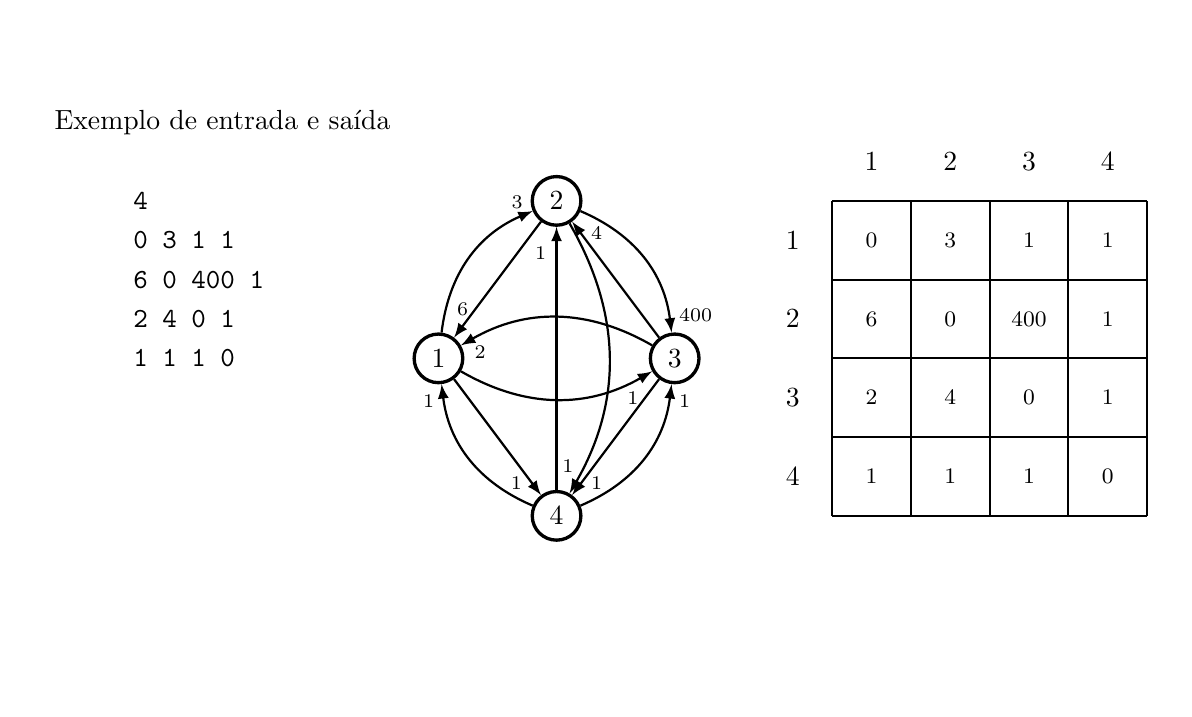
\begin{tikzpicture}
\node[draw,opacity=0] at (0, 0) {x};
\node[draw,opacity=0] at (14, 8) {x};

	\node[anchor=west] (header) at (0, 7.0) { \bbbold{Exemplo de entrada e saída} };


	\node[anchor=west] (line1) at (1.0, 6.0) { \bbtext{\texttt{4} } };


	\node[draw,very thick,circle] (node1) at (5.0, 4.0) { \bbtext{1} };

	\node[draw,very thick,circle] (node2) at (6.5, 6.0) { \bbtext{2} };

	\node[draw,very thick,circle] (node3) at (8.0, 4.0) { \bbtext{3} };

	\node[draw,very thick,circle] (node4) at (6.5, 2.0) { \bbtext{4} };


	\node[anchor=west] (line2) at (1.0, 5.5) { \bbtext{\texttt{0 3 1 1} } };

	\node[anchor=west] (line3) at (1.0, 5.0) { \bbtext{\texttt{6 0 400 1} } };

	\node[anchor=west] (line4) at (1.0, 4.5) { \bbtext{\texttt{2 4 0 1} } };

	\node[anchor=west] (line5) at (1.0, 4.0) { \bbtext{\texttt{1 1 1 0} } };


	\draw[thick] (10.0, 2.0) grid  (14.0, 6.0);

	\node[] (c1) at (9.5, 5.5) { \bbtext{1} };

	\node[] (c2) at (9.5, 4.5) { \bbtext{2} };

	\node[] (c3) at (9.5, 3.5) { \bbtext{3} };

	\node[] (c4) at (9.5, 2.5) { \bbtext{4} };

	\node[] (r1) at (10.5, 6.5) { \bbtext{1} };

	\node[] (r2) at (11.5, 6.5) { \bbtext{2} };

	\node[] (r3) at (12.5, 6.5) { \bbtext{3} };

	\node[] (r4) at (13.5, 6.5) { \bbtext{4} };

	\node[] (a11) at (10.5, 5.5) { \footnotesize $0$ };

	\node[] (a12) at (11.5, 5.5) { \footnotesize $3$ };

	\node[] (a13) at (12.5, 5.5) { \footnotesize $1$ };

	\node[] (a14) at (13.5, 5.5) { \footnotesize $1$ };

	\node[] (a21) at (10.5, 4.5) { \footnotesize $6$ };

	\node[] (a22) at (11.5, 4.5) { \footnotesize $0$ };

	\node[] (a23) at (12.5, 4.5) { \footnotesize $400$ };

	\node[] (a24) at (13.5, 4.5) { \footnotesize $1$ };

	\node[] (a31) at (10.5, 3.5) { \footnotesize $2$ };

	\node[] (a32) at (11.5, 3.5) { \footnotesize $4$ };

	\node[] (a33) at (12.5, 3.5) { \footnotesize $0$ };

	\node[] (a34) at (13.5, 3.5) { \footnotesize $1$ };

	\node[] (a41) at (10.5, 2.5) { \footnotesize $1$ };

	\node[] (a42) at (11.5, 2.5) { \footnotesize $1$ };

	\node[] (a43) at (12.5, 2.5) { \footnotesize $1$ };

	\node[] (a44) at (13.5, 2.5) { \footnotesize $0$ };

	\draw[-latex,thick](node1) to [bend left] node[above,pos=0.9] { \scriptsize \bbinfo{3} } (node2);

	\draw[-latex,thick](node1) to [bend right] node[below,pos=0.9] { \scriptsize \bbinfo{1} } (node3);

	\draw[-latex,thick](node1) to node[left,pos=0.9] { \scriptsize \bbinfo{1} } (node4);

	\draw[-latex,thick](node2) to node[above,pos=0.9] { \scriptsize \bbinfo{6} } (node1);

	\draw[-latex,thick](node2) to [bend left] node[right,pos=0.9] { \scriptsize \bbinfo{400} } (node3);

	\draw[-latex,thick](node2) to [bend left] node[left,pos=0.9] { \scriptsize \bbinfo{1} } (node4);

	\draw[-latex,thick](node3) to [bend right] node[below,pos=0.9] { \scriptsize \bbinfo{2} } (node1);

	\draw[-latex,thick](node3) to node[right,pos=0.9] { \scriptsize \bbinfo{4} } (node2);

	\draw[-latex,thick](node3) to node[right,pos=0.9] { \scriptsize \bbinfo{1} } (node4);

	\draw[-latex,thick](node4) to [bend left] node[left,pos=0.9] { \scriptsize \bbinfo{1} } (node1);

	\draw[-latex,thick](node4) to node[left,pos=0.9] { \scriptsize \bbinfo{1} } (node2);

	\draw[-latex,thick](node4) to [bend right] node[right,pos=0.9] { \scriptsize \bbinfo{1} } (node3);


\end{tikzpicture}
\end{frame}
\begin{frame}[plain,t]
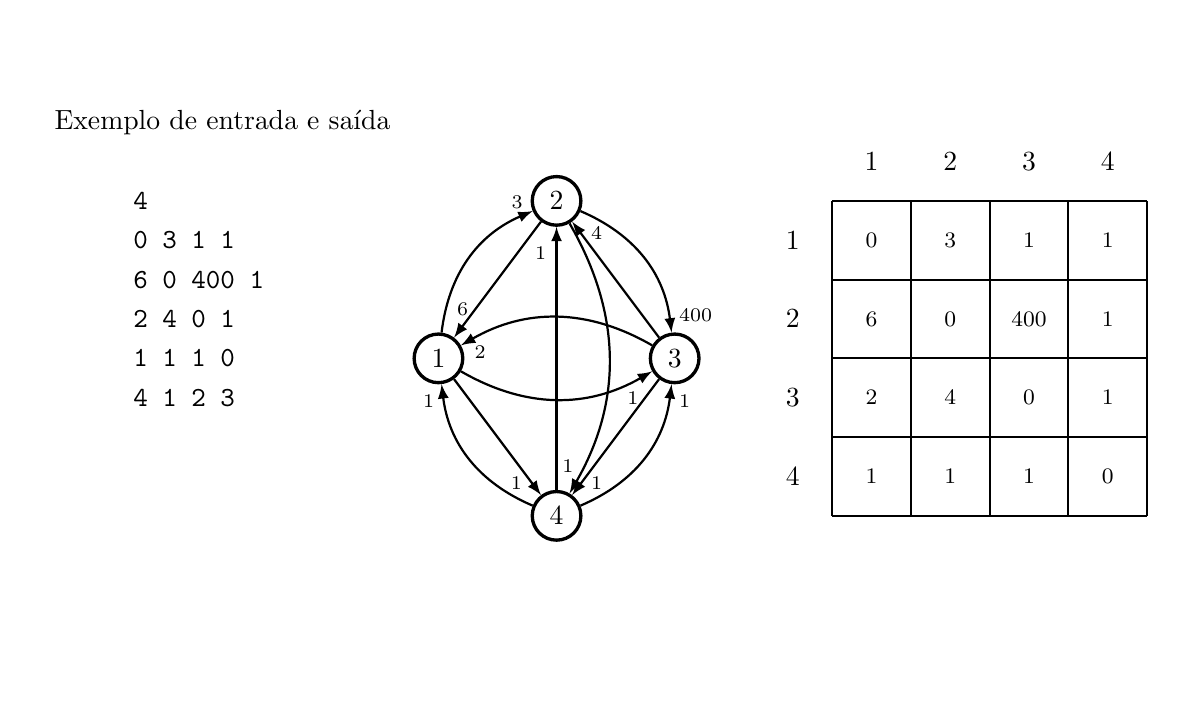
\begin{tikzpicture}
\node[draw,opacity=0] at (0, 0) {x};
\node[draw,opacity=0] at (14, 8) {x};

	\node[anchor=west] (header) at (0, 7.0) { \bbbold{Exemplo de entrada e saída} };


	\node[anchor=west] (line1) at (1.0, 6.0) { \bbtext{\texttt{4} } };


	\node[draw,very thick,circle] (node1) at (5.0, 4.0) { \bbtext{1} };

	\node[draw,very thick,circle] (node2) at (6.5, 6.0) { \bbtext{2} };

	\node[draw,very thick,circle] (node3) at (8.0, 4.0) { \bbtext{3} };

	\node[draw,very thick,circle] (node4) at (6.5, 2.0) { \bbtext{4} };


	\node[anchor=west] (line2) at (1.0, 5.5) { \bbtext{\texttt{0 3 1 1} } };

	\node[anchor=west] (line3) at (1.0, 5.0) { \bbtext{\texttt{6 0 400 1} } };

	\node[anchor=west] (line4) at (1.0, 4.5) { \bbtext{\texttt{2 4 0 1} } };

	\node[anchor=west] (line5) at (1.0, 4.0) { \bbtext{\texttt{1 1 1 0} } };


	\draw[thick] (10.0, 2.0) grid  (14.0, 6.0);

	\node[] (c1) at (9.5, 5.5) { \bbtext{1} };

	\node[] (c2) at (9.5, 4.5) { \bbtext{2} };

	\node[] (c3) at (9.5, 3.5) { \bbtext{3} };

	\node[] (c4) at (9.5, 2.5) { \bbtext{4} };

	\node[] (r1) at (10.5, 6.5) { \bbtext{1} };

	\node[] (r2) at (11.5, 6.5) { \bbtext{2} };

	\node[] (r3) at (12.5, 6.5) { \bbtext{3} };

	\node[] (r4) at (13.5, 6.5) { \bbtext{4} };

	\node[] (a11) at (10.5, 5.5) { \footnotesize $0$ };

	\node[] (a12) at (11.5, 5.5) { \footnotesize $3$ };

	\node[] (a13) at (12.5, 5.5) { \footnotesize $1$ };

	\node[] (a14) at (13.5, 5.5) { \footnotesize $1$ };

	\node[] (a21) at (10.5, 4.5) { \footnotesize $6$ };

	\node[] (a22) at (11.5, 4.5) { \footnotesize $0$ };

	\node[] (a23) at (12.5, 4.5) { \footnotesize $400$ };

	\node[] (a24) at (13.5, 4.5) { \footnotesize $1$ };

	\node[] (a31) at (10.5, 3.5) { \footnotesize $2$ };

	\node[] (a32) at (11.5, 3.5) { \footnotesize $4$ };

	\node[] (a33) at (12.5, 3.5) { \footnotesize $0$ };

	\node[] (a34) at (13.5, 3.5) { \footnotesize $1$ };

	\node[] (a41) at (10.5, 2.5) { \footnotesize $1$ };

	\node[] (a42) at (11.5, 2.5) { \footnotesize $1$ };

	\node[] (a43) at (12.5, 2.5) { \footnotesize $1$ };

	\node[] (a44) at (13.5, 2.5) { \footnotesize $0$ };

	\draw[-latex,thick](node1) to [bend left] node[above,pos=0.9] { \scriptsize \bbinfo{3} } (node2);

	\draw[-latex,thick](node1) to [bend right] node[below,pos=0.9] { \scriptsize \bbinfo{1} } (node3);

	\draw[-latex,thick](node1) to node[left,pos=0.9] { \scriptsize \bbinfo{1} } (node4);

	\draw[-latex,thick](node2) to node[above,pos=0.9] { \scriptsize \bbinfo{6} } (node1);

	\draw[-latex,thick](node2) to [bend left] node[right,pos=0.9] { \scriptsize \bbinfo{400} } (node3);

	\draw[-latex,thick](node2) to [bend left] node[left,pos=0.9] { \scriptsize \bbinfo{1} } (node4);

	\draw[-latex,thick](node3) to [bend right] node[below,pos=0.9] { \scriptsize \bbinfo{2} } (node1);

	\draw[-latex,thick](node3) to node[right,pos=0.9] { \scriptsize \bbinfo{4} } (node2);

	\draw[-latex,thick](node3) to node[right,pos=0.9] { \scriptsize \bbinfo{1} } (node4);

	\draw[-latex,thick](node4) to [bend left] node[left,pos=0.9] { \scriptsize \bbinfo{1} } (node1);

	\draw[-latex,thick](node4) to node[left,pos=0.9] { \scriptsize \bbinfo{1} } (node2);

	\draw[-latex,thick](node4) to [bend right] node[right,pos=0.9] { \scriptsize \bbinfo{1} } (node3);



	\node[anchor=west] (line6) at (1.0, 3.5) { \bbtext{\texttt{4 1 2 3} } };

\end{tikzpicture}
\end{frame}
\begin{frame}[plain,t]
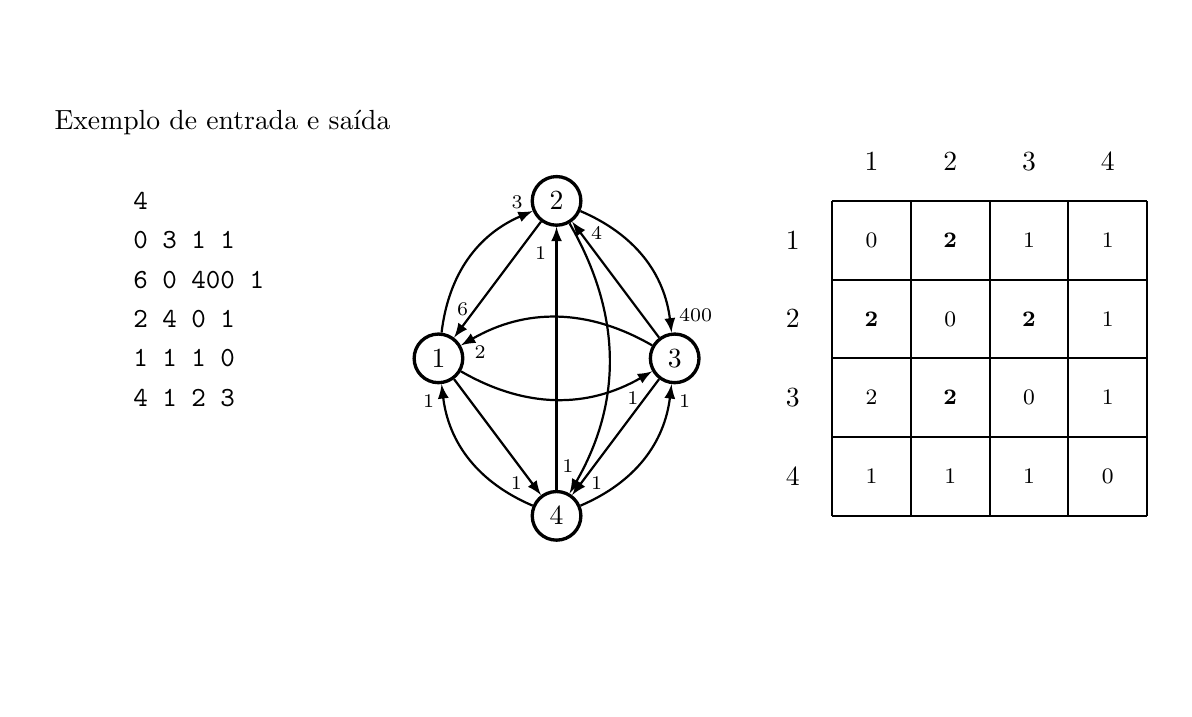
\begin{tikzpicture}
\node[draw,opacity=0] at (0, 0) {x};
\node[draw,opacity=0] at (14, 8) {x};

	\node[anchor=west] (header) at (0, 7.0) { \bbbold{Exemplo de entrada e saída} };


	\node[anchor=west] (line1) at (1.0, 6.0) { \bbtext{\texttt{4} } };


	\node[draw,very thick,circle] (node1) at (5.0, 4.0) { \bbtext{1} };

	\node[draw,very thick,circle] (node2) at (6.5, 6.0) { \bbtext{2} };

	\node[draw,very thick,circle] (node3) at (8.0, 4.0) { \bbtext{3} };

	\node[draw,very thick,circle] (node4) at (6.5, 2.0) { \bbtext{4} };


	\node[anchor=west] (line2) at (1.0, 5.5) { \bbtext{\texttt{0 3 1 1} } };

	\node[anchor=west] (line3) at (1.0, 5.0) { \bbtext{\texttt{6 0 400 1} } };

	\node[anchor=west] (line4) at (1.0, 4.5) { \bbtext{\texttt{2 4 0 1} } };

	\node[anchor=west] (line5) at (1.0, 4.0) { \bbtext{\texttt{1 1 1 0} } };


	\draw[thick] (10.0, 2.0) grid  (14.0, 6.0);

	\node[] (c1) at (9.5, 5.5) { \bbtext{1} };

	\node[] (c2) at (9.5, 4.5) { \bbtext{2} };

	\node[] (c3) at (9.5, 3.5) { \bbtext{3} };

	\node[] (c4) at (9.5, 2.5) { \bbtext{4} };

	\node[] (r1) at (10.5, 6.5) { \bbtext{1} };

	\node[] (r2) at (11.5, 6.5) { \bbtext{2} };

	\node[] (r3) at (12.5, 6.5) { \bbtext{3} };

	\node[] (r4) at (13.5, 6.5) { \bbtext{4} };

	\node[] (a11) at (10.5, 5.5) { \footnotesize $0$ };

	\node[] (a12) at (11.5, 5.5) { \footnotesize $\mathbf{2}$ };

	\node[] (a13) at (12.5, 5.5) { \footnotesize $1$ };

	\node[] (a14) at (13.5, 5.5) { \footnotesize $1$ };

	\node[] (a21) at (10.5, 4.5) { \footnotesize $\mathbf{2}$ };

	\node[] (a22) at (11.5, 4.5) { \footnotesize $0$ };

	\node[] (a23) at (12.5, 4.5) { \footnotesize $\mathbf{2}$ };

	\node[] (a24) at (13.5, 4.5) { \footnotesize $1$ };

	\node[] (a31) at (10.5, 3.5) { \footnotesize $2$ };

	\node[] (a32) at (11.5, 3.5) { \footnotesize $\mathbf{2}$ };

	\node[] (a33) at (12.5, 3.5) { \footnotesize $0$ };

	\node[] (a34) at (13.5, 3.5) { \footnotesize $1$ };

	\node[] (a41) at (10.5, 2.5) { \footnotesize $1$ };

	\node[] (a42) at (11.5, 2.5) { \footnotesize $1$ };

	\node[] (a43) at (12.5, 2.5) { \footnotesize $1$ };

	\node[] (a44) at (13.5, 2.5) { \footnotesize $0$ };

	\draw[-latex,thick](node1) to [bend left] node[above,pos=0.9] { \scriptsize \bbinfo{3} } (node2);

	\draw[-latex,thick](node1) to [bend right] node[below,pos=0.9] { \scriptsize \bbinfo{1} } (node3);

	\draw[-latex,thick](node1) to node[left,pos=0.9] { \scriptsize \bbinfo{1} } (node4);

	\draw[-latex,thick](node2) to node[above,pos=0.9] { \scriptsize \bbinfo{6} } (node1);

	\draw[-latex,thick](node2) to [bend left] node[right,pos=0.9] { \scriptsize \bbinfo{400} } (node3);

	\draw[-latex,thick](node2) to [bend left] node[left,pos=0.9] { \scriptsize \bbinfo{1} } (node4);

	\draw[-latex,thick](node3) to [bend right] node[below,pos=0.9] { \scriptsize \bbinfo{2} } (node1);

	\draw[-latex,thick](node3) to node[right,pos=0.9] { \scriptsize \bbinfo{4} } (node2);

	\draw[-latex,thick](node3) to node[right,pos=0.9] { \scriptsize \bbinfo{1} } (node4);

	\draw[-latex,thick](node4) to [bend left] node[left,pos=0.9] { \scriptsize \bbinfo{1} } (node1);

	\draw[-latex,thick](node4) to node[left,pos=0.9] { \scriptsize \bbinfo{1} } (node2);

	\draw[-latex,thick](node4) to [bend right] node[right,pos=0.9] { \scriptsize \bbinfo{1} } (node3);



	\node[anchor=west] (line6) at (1.0, 3.5) { \bbtext{\texttt{4 1 2 3} } };



\end{tikzpicture}
\end{frame}
\begin{frame}[plain,t]
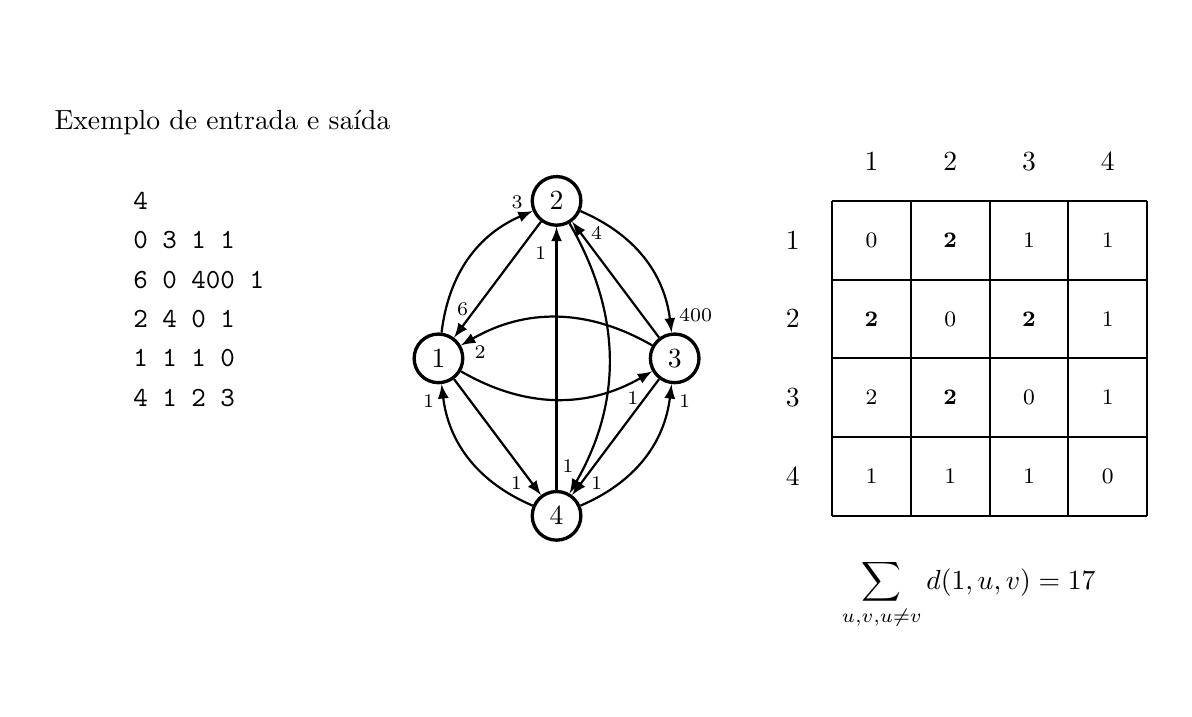
\begin{tikzpicture}
\node[draw,opacity=0] at (0, 0) {x};
\node[draw,opacity=0] at (14, 8) {x};

	\node[anchor=west] (header) at (0, 7.0) { \bbbold{Exemplo de entrada e saída} };


	\node[anchor=west] (line1) at (1.0, 6.0) { \bbtext{\texttt{4} } };


	\node[draw,very thick,circle] (node1) at (5.0, 4.0) { \bbtext{1} };

	\node[draw,very thick,circle] (node2) at (6.5, 6.0) { \bbtext{2} };

	\node[draw,very thick,circle] (node3) at (8.0, 4.0) { \bbtext{3} };

	\node[draw,very thick,circle] (node4) at (6.5, 2.0) { \bbtext{4} };


	\node[anchor=west] (line2) at (1.0, 5.5) { \bbtext{\texttt{0 3 1 1} } };

	\node[anchor=west] (line3) at (1.0, 5.0) { \bbtext{\texttt{6 0 400 1} } };

	\node[anchor=west] (line4) at (1.0, 4.5) { \bbtext{\texttt{2 4 0 1} } };

	\node[anchor=west] (line5) at (1.0, 4.0) { \bbtext{\texttt{1 1 1 0} } };


	\draw[thick] (10.0, 2.0) grid  (14.0, 6.0);

	\node[] (c1) at (9.5, 5.5) { \bbtext{1} };

	\node[] (c2) at (9.5, 4.5) { \bbtext{2} };

	\node[] (c3) at (9.5, 3.5) { \bbtext{3} };

	\node[] (c4) at (9.5, 2.5) { \bbtext{4} };

	\node[] (r1) at (10.5, 6.5) { \bbtext{1} };

	\node[] (r2) at (11.5, 6.5) { \bbtext{2} };

	\node[] (r3) at (12.5, 6.5) { \bbtext{3} };

	\node[] (r4) at (13.5, 6.5) { \bbtext{4} };

	\node[] (a11) at (10.5, 5.5) { \footnotesize $0$ };

	\node[] (a12) at (11.5, 5.5) { \footnotesize $\mathbf{2}$ };

	\node[] (a13) at (12.5, 5.5) { \footnotesize $1$ };

	\node[] (a14) at (13.5, 5.5) { \footnotesize $1$ };

	\node[] (a21) at (10.5, 4.5) { \footnotesize $\mathbf{2}$ };

	\node[] (a22) at (11.5, 4.5) { \footnotesize $0$ };

	\node[] (a23) at (12.5, 4.5) { \footnotesize $\mathbf{2}$ };

	\node[] (a24) at (13.5, 4.5) { \footnotesize $1$ };

	\node[] (a31) at (10.5, 3.5) { \footnotesize $2$ };

	\node[] (a32) at (11.5, 3.5) { \footnotesize $\mathbf{2}$ };

	\node[] (a33) at (12.5, 3.5) { \footnotesize $0$ };

	\node[] (a34) at (13.5, 3.5) { \footnotesize $1$ };

	\node[] (a41) at (10.5, 2.5) { \footnotesize $1$ };

	\node[] (a42) at (11.5, 2.5) { \footnotesize $1$ };

	\node[] (a43) at (12.5, 2.5) { \footnotesize $1$ };

	\node[] (a44) at (13.5, 2.5) { \footnotesize $0$ };

	\draw[-latex,thick](node1) to [bend left] node[above,pos=0.9] { \scriptsize \bbinfo{3} } (node2);

	\draw[-latex,thick](node1) to [bend right] node[below,pos=0.9] { \scriptsize \bbinfo{1} } (node3);

	\draw[-latex,thick](node1) to node[left,pos=0.9] { \scriptsize \bbinfo{1} } (node4);

	\draw[-latex,thick](node2) to node[above,pos=0.9] { \scriptsize \bbinfo{6} } (node1);

	\draw[-latex,thick](node2) to [bend left] node[right,pos=0.9] { \scriptsize \bbinfo{400} } (node3);

	\draw[-latex,thick](node2) to [bend left] node[left,pos=0.9] { \scriptsize \bbinfo{1} } (node4);

	\draw[-latex,thick](node3) to [bend right] node[below,pos=0.9] { \scriptsize \bbinfo{2} } (node1);

	\draw[-latex,thick](node3) to node[right,pos=0.9] { \scriptsize \bbinfo{4} } (node2);

	\draw[-latex,thick](node3) to node[right,pos=0.9] { \scriptsize \bbinfo{1} } (node4);

	\draw[-latex,thick](node4) to [bend left] node[left,pos=0.9] { \scriptsize \bbinfo{1} } (node1);

	\draw[-latex,thick](node4) to node[left,pos=0.9] { \scriptsize \bbinfo{1} } (node2);

	\draw[-latex,thick](node4) to [bend right] node[right,pos=0.9] { \scriptsize \bbinfo{1} } (node3);



	\node[anchor=west] (line6) at (1.0, 3.5) { \bbtext{\texttt{4 1 2 3} } };




	\node[anchor=west] (eq) at (10.0, 1.0) { $\displaystyle \sum_{u, v, u\neq v} d(1, u, v) = 17$ };

\end{tikzpicture}
\end{frame}
\begin{frame}[plain,t]
\begin{tikzpicture}
\node[draw,opacity=0] at (0, 0) {x};
\node[draw,opacity=0] at (14, 8) {x};

	\node[anchor=west] (header) at (0, 7.0) { \bbbold{Exemplo de entrada e saída} };


	\node[anchor=west] (line1) at (1.0, 6.0) { \bbtext{\texttt{4} } };


	\node[draw,very thick,circle] (node1) at (5.0, 4.0) { \bbtext{1} };

	\node[draw,very thick,circle] (node2) at (6.5, 6.0) { \bbtext{2} };

	\node[draw,very thick,circle] (node3) at (8.0, 4.0) { \bbtext{3} };

	\node[draw,very thick,circle,fill=BBRed] (node4) at (6.5, 2.0) { \bbtext{4} };


	\node[anchor=west] (line2) at (1.0, 5.5) { \bbtext{\texttt{0 3 1 1} } };

	\node[anchor=west] (line3) at (1.0, 5.0) { \bbtext{\texttt{6 0 400 1} } };

	\node[anchor=west] (line4) at (1.0, 4.5) { \bbtext{\texttt{2 4 0 1} } };

	\node[anchor=west] (line5) at (1.0, 4.0) { \bbtext{\texttt{1 1 1 0} } };


	\draw[thick] (10.0, 2.0) grid  (14.0, 6.0);

	\node[] (c1) at (9.5, 5.5) { \bbtext{1} };

	\node[] (c2) at (9.5, 4.5) { \bbtext{2} };

	\node[] (c3) at (9.5, 3.5) { \bbtext{3} };

	\node[] (c4) at (9.5, 2.5) { \bbtext{4} };

	\node[] (r1) at (10.5, 6.5) { \bbtext{1} };

	\node[] (r2) at (11.5, 6.5) { \bbtext{2} };

	\node[] (r3) at (12.5, 6.5) { \bbtext{3} };

	\node[] (r4) at (13.5, 6.5) { \bbtext{4} };

	\node[] (a11) at (10.5, 5.5) { \footnotesize $0$ };

	\node[] (a12) at (11.5, 5.5) { \footnotesize ${2}$ };

	\node[] (a13) at (12.5, 5.5) { \footnotesize $1$ };

	\node[] (a14) at (13.5, 5.5) { \footnotesize $1$ };

	\node[] (a21) at (10.5, 4.5) { \footnotesize ${2}$ };

	\node[] (a22) at (11.5, 4.5) { \footnotesize $0$ };

	\node[] (a23) at (12.5, 4.5) { \footnotesize ${2}$ };

	\node[] (a24) at (13.5, 4.5) { \footnotesize $1$ };

	\node[] (a31) at (10.5, 3.5) { \footnotesize $2$ };

	\node[] (a32) at (11.5, 3.5) { \footnotesize ${2}$ };

	\node[] (a33) at (12.5, 3.5) { \footnotesize $0$ };

	\node[] (a34) at (13.5, 3.5) { \footnotesize $1$ };

	\node[] (a41) at (10.5, 2.5) { \footnotesize $1$ };

	\node[] (a42) at (11.5, 2.5) { \footnotesize $1$ };

	\node[] (a43) at (12.5, 2.5) { \footnotesize $1$ };

	\node[] (a44) at (13.5, 2.5) { \footnotesize $0$ };

	\draw[-latex,thick](node1) to [bend left] node[above,pos=0.9] { \scriptsize \bbinfo{3} } (node2);

	\draw[-latex,thick](node1) to [bend right] node[below,pos=0.9] { \scriptsize \bbinfo{1} } (node3);

	\draw[-latex,thick](node1) to node[left,pos=0.9] { \scriptsize \bbinfo{1} } (node4);

	\draw[-latex,thick](node2) to node[above,pos=0.9] { \scriptsize \bbinfo{6} } (node1);

	\draw[-latex,thick](node2) to [bend left] node[right,pos=0.9] { \scriptsize \bbinfo{400} } (node3);

	\draw[-latex,thick](node2) to [bend left] node[left,pos=0.9] { \scriptsize \bbinfo{1} } (node4);

	\draw[-latex,thick](node3) to [bend right] node[below,pos=0.9] { \scriptsize \bbinfo{2} } (node1);

	\draw[-latex,thick](node3) to node[right,pos=0.9] { \scriptsize \bbinfo{4} } (node2);

	\draw[-latex,thick](node3) to node[right,pos=0.9] { \scriptsize \bbinfo{1} } (node4);

	\draw[-latex,thick](node4) to [bend left] node[left,pos=0.9] { \scriptsize \bbinfo{1} } (node1);

	\draw[-latex,thick](node4) to node[left,pos=0.9] { \scriptsize \bbinfo{1} } (node2);

	\draw[-latex,thick](node4) to [bend right] node[right,pos=0.9] { \scriptsize \bbinfo{1} } (node3);



	\node[anchor=west] (line6) at (1.0, 3.5) { \bbtext{\texttt{4 1 2 3} } };








\end{tikzpicture}
\end{frame}
\begin{frame}[plain,t]
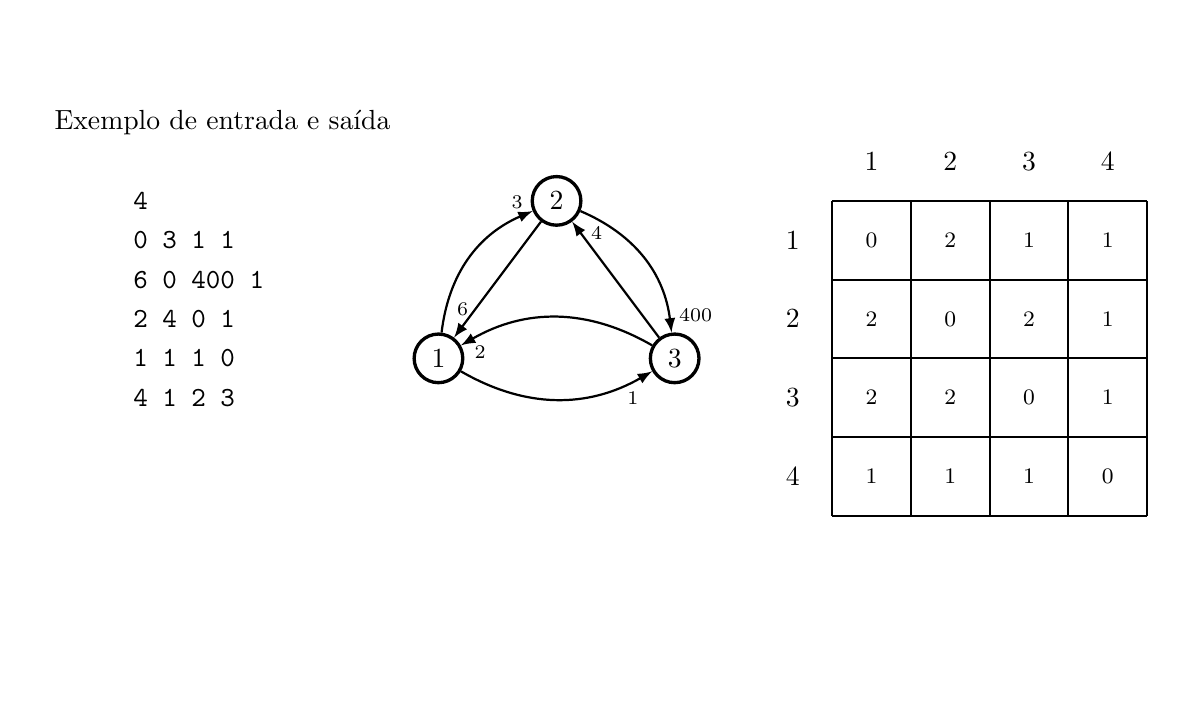
\begin{tikzpicture}
\node[draw,opacity=0] at (0, 0) {x};
\node[draw,opacity=0] at (14, 8) {x};

	\node[anchor=west] (header) at (0, 7.0) { \bbbold{Exemplo de entrada e saída} };


	\node[anchor=west] (line1) at (1.0, 6.0) { \bbtext{\texttt{4} } };


	\node[draw,very thick,circle] (node1) at (5.0, 4.0) { \bbtext{1} };

	\node[draw,very thick,circle] (node2) at (6.5, 6.0) { \bbtext{2} };

	\node[draw,very thick,circle] (node3) at (8.0, 4.0) { \bbtext{3} };



	\node[anchor=west] (line2) at (1.0, 5.5) { \bbtext{\texttt{0 3 1 1} } };

	\node[anchor=west] (line3) at (1.0, 5.0) { \bbtext{\texttt{6 0 400 1} } };

	\node[anchor=west] (line4) at (1.0, 4.5) { \bbtext{\texttt{2 4 0 1} } };

	\node[anchor=west] (line5) at (1.0, 4.0) { \bbtext{\texttt{1 1 1 0} } };


	\draw[thick] (10.0, 2.0) grid  (14.0, 6.0);

	\node[] (c1) at (9.5, 5.5) { \bbtext{1} };

	\node[] (c2) at (9.5, 4.5) { \bbtext{2} };

	\node[] (c3) at (9.5, 3.5) { \bbtext{3} };

	\node[] (c4) at (9.5, 2.5) { \bbtext{4} };

	\node[] (r1) at (10.5, 6.5) { \bbtext{1} };

	\node[] (r2) at (11.5, 6.5) { \bbtext{2} };

	\node[] (r3) at (12.5, 6.5) { \bbtext{3} };

	\node[] (r4) at (13.5, 6.5) { \bbtext{4} };

	\node[] (a11) at (10.5, 5.5) { \footnotesize $0$ };

	\node[] (a12) at (11.5, 5.5) { \footnotesize ${2}$ };

	\node[] (a13) at (12.5, 5.5) { \footnotesize $1$ };

	\node[] (a14) at (13.5, 5.5) { \footnotesize $1$ };

	\node[] (a21) at (10.5, 4.5) { \footnotesize ${2}$ };

	\node[] (a22) at (11.5, 4.5) { \footnotesize $0$ };

	\node[] (a23) at (12.5, 4.5) { \footnotesize ${2}$ };

	\node[] (a24) at (13.5, 4.5) { \footnotesize $1$ };

	\node[] (a31) at (10.5, 3.5) { \footnotesize $2$ };

	\node[] (a32) at (11.5, 3.5) { \footnotesize ${2}$ };

	\node[] (a33) at (12.5, 3.5) { \footnotesize $0$ };

	\node[] (a34) at (13.5, 3.5) { \footnotesize $1$ };

	\node[] (a41) at (10.5, 2.5) { \footnotesize $1$ };

	\node[] (a42) at (11.5, 2.5) { \footnotesize $1$ };

	\node[] (a43) at (12.5, 2.5) { \footnotesize $1$ };

	\node[] (a44) at (13.5, 2.5) { \footnotesize $0$ };

	\draw[-latex,thick](node1) to [bend left] node[above,pos=0.9] { \scriptsize \bbinfo{3} } (node2);

	\draw[-latex,thick](node1) to [bend right] node[below,pos=0.9] { \scriptsize \bbinfo{1} } (node3);


	\draw[-latex,thick](node2) to node[above,pos=0.9] { \scriptsize \bbinfo{6} } (node1);

	\draw[-latex,thick](node2) to [bend left] node[right,pos=0.9] { \scriptsize \bbinfo{400} } (node3);


	\draw[-latex,thick](node3) to [bend right] node[below,pos=0.9] { \scriptsize \bbinfo{2} } (node1);

	\draw[-latex,thick](node3) to node[right,pos=0.9] { \scriptsize \bbinfo{4} } (node2);







	\node[anchor=west] (line6) at (1.0, 3.5) { \bbtext{\texttt{4 1 2 3} } };










\end{tikzpicture}
\end{frame}
\begin{frame}[plain,t]
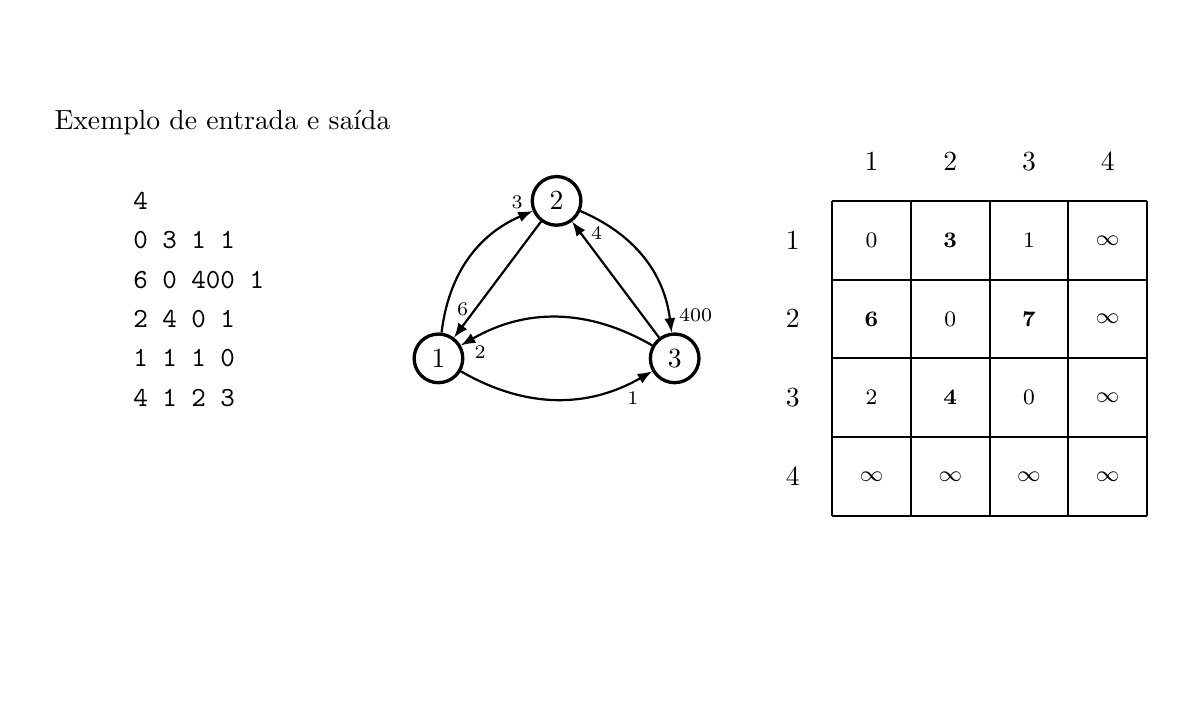
\begin{tikzpicture}
\node[draw,opacity=0] at (0, 0) {x};
\node[draw,opacity=0] at (14, 8) {x};

	\node[anchor=west] (header) at (0, 7.0) { \bbbold{Exemplo de entrada e saída} };


	\node[anchor=west] (line1) at (1.0, 6.0) { \bbtext{\texttt{4} } };


	\node[draw,very thick,circle] (node1) at (5.0, 4.0) { \bbtext{1} };

	\node[draw,very thick,circle] (node2) at (6.5, 6.0) { \bbtext{2} };

	\node[draw,very thick,circle] (node3) at (8.0, 4.0) { \bbtext{3} };



	\node[anchor=west] (line2) at (1.0, 5.5) { \bbtext{\texttt{0 3 1 1} } };

	\node[anchor=west] (line3) at (1.0, 5.0) { \bbtext{\texttt{6 0 400 1} } };

	\node[anchor=west] (line4) at (1.0, 4.5) { \bbtext{\texttt{2 4 0 1} } };

	\node[anchor=west] (line5) at (1.0, 4.0) { \bbtext{\texttt{1 1 1 0} } };


	\draw[thick] (10.0, 2.0) grid  (14.0, 6.0);

	\node[] (c1) at (9.5, 5.5) { \bbtext{1} };

	\node[] (c2) at (9.5, 4.5) { \bbtext{2} };

	\node[] (c3) at (9.5, 3.5) { \bbtext{3} };

	\node[] (c4) at (9.5, 2.5) { \bbtext{4} };

	\node[] (r1) at (10.5, 6.5) { \bbtext{1} };

	\node[] (r2) at (11.5, 6.5) { \bbtext{2} };

	\node[] (r3) at (12.5, 6.5) { \bbtext{3} };

	\node[] (r4) at (13.5, 6.5) { \bbtext{4} };

	\node[] (a11) at (10.5, 5.5) { \footnotesize $0$ };

	\node[] (a12) at (11.5, 5.5) { \footnotesize $\mathbf{3}$ };

	\node[] (a13) at (12.5, 5.5) { \footnotesize $1$ };

	\node[] (a14) at (13.5, 5.5) { \footnotesize $\infty$ };

	\node[] (a21) at (10.5, 4.5) { \footnotesize $\mathbf{6}$ };

	\node[] (a22) at (11.5, 4.5) { \footnotesize $0$ };

	\node[] (a23) at (12.5, 4.5) { \footnotesize $\mathbf{7}$ };

	\node[] (a24) at (13.5, 4.5) { \footnotesize $\infty$ };

	\node[] (a31) at (10.5, 3.5) { \footnotesize $2$ };

	\node[] (a32) at (11.5, 3.5) { \footnotesize $\mathbf{4}$ };

	\node[] (a33) at (12.5, 3.5) { \footnotesize $0$ };

	\node[] (a34) at (13.5, 3.5) { \footnotesize $\infty$ };

	\node[] (a41) at (10.5, 2.5) { \footnotesize $\infty$ };

	\node[] (a42) at (11.5, 2.5) { \footnotesize $\infty$ };

	\node[] (a43) at (12.5, 2.5) { \footnotesize $\infty$ };

	\node[] (a44) at (13.5, 2.5) { \footnotesize $\infty$ };

	\draw[-latex,thick](node1) to [bend left] node[above,pos=0.9] { \scriptsize \bbinfo{3} } (node2);

	\draw[-latex,thick](node1) to [bend right] node[below,pos=0.9] { \scriptsize \bbinfo{1} } (node3);


	\draw[-latex,thick](node2) to node[above,pos=0.9] { \scriptsize \bbinfo{6} } (node1);

	\draw[-latex,thick](node2) to [bend left] node[right,pos=0.9] { \scriptsize \bbinfo{400} } (node3);


	\draw[-latex,thick](node3) to [bend right] node[below,pos=0.9] { \scriptsize \bbinfo{2} } (node1);

	\draw[-latex,thick](node3) to node[right,pos=0.9] { \scriptsize \bbinfo{4} } (node2);







	\node[anchor=west] (line6) at (1.0, 3.5) { \bbtext{\texttt{4 1 2 3} } };












\end{tikzpicture}
\end{frame}
\begin{frame}[plain,t]
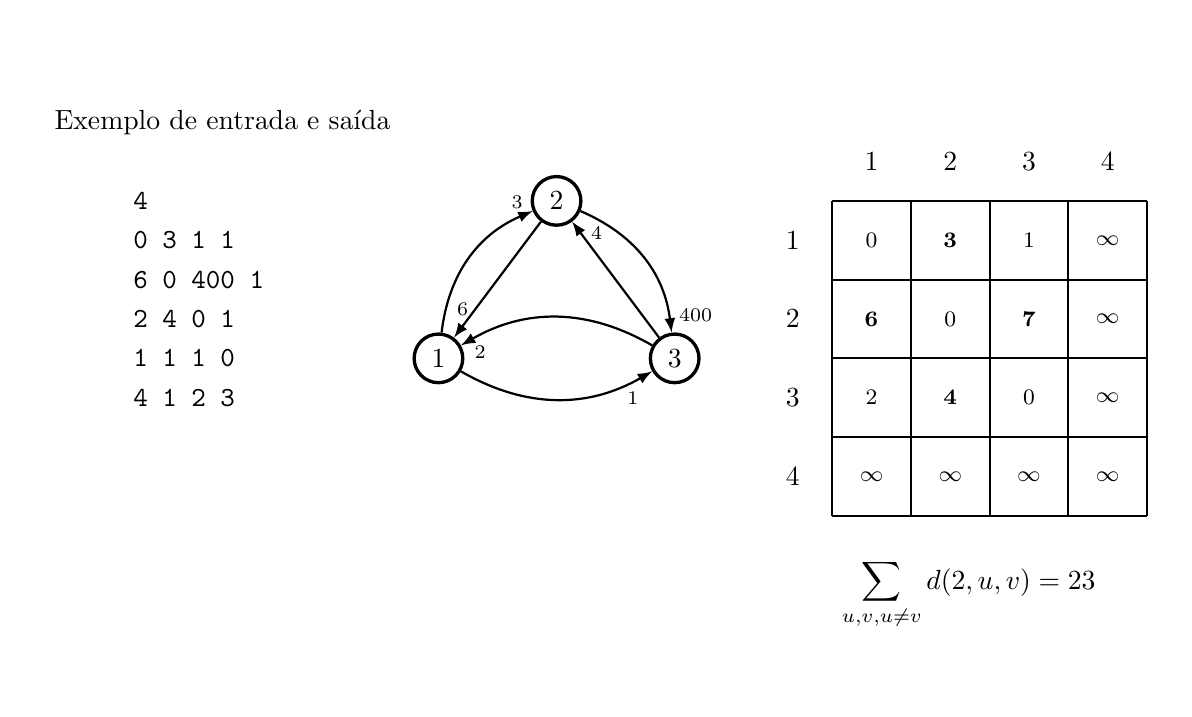
\begin{tikzpicture}
\node[draw,opacity=0] at (0, 0) {x};
\node[draw,opacity=0] at (14, 8) {x};

	\node[anchor=west] (header) at (0, 7.0) { \bbbold{Exemplo de entrada e saída} };


	\node[anchor=west] (line1) at (1.0, 6.0) { \bbtext{\texttt{4} } };


	\node[draw,very thick,circle] (node1) at (5.0, 4.0) { \bbtext{1} };

	\node[draw,very thick,circle] (node2) at (6.5, 6.0) { \bbtext{2} };

	\node[draw,very thick,circle] (node3) at (8.0, 4.0) { \bbtext{3} };



	\node[anchor=west] (line2) at (1.0, 5.5) { \bbtext{\texttt{0 3 1 1} } };

	\node[anchor=west] (line3) at (1.0, 5.0) { \bbtext{\texttt{6 0 400 1} } };

	\node[anchor=west] (line4) at (1.0, 4.5) { \bbtext{\texttt{2 4 0 1} } };

	\node[anchor=west] (line5) at (1.0, 4.0) { \bbtext{\texttt{1 1 1 0} } };


	\draw[thick] (10.0, 2.0) grid  (14.0, 6.0);

	\node[] (c1) at (9.5, 5.5) { \bbtext{1} };

	\node[] (c2) at (9.5, 4.5) { \bbtext{2} };

	\node[] (c3) at (9.5, 3.5) { \bbtext{3} };

	\node[] (c4) at (9.5, 2.5) { \bbtext{4} };

	\node[] (r1) at (10.5, 6.5) { \bbtext{1} };

	\node[] (r2) at (11.5, 6.5) { \bbtext{2} };

	\node[] (r3) at (12.5, 6.5) { \bbtext{3} };

	\node[] (r4) at (13.5, 6.5) { \bbtext{4} };

	\node[] (a11) at (10.5, 5.5) { \footnotesize $0$ };

	\node[] (a12) at (11.5, 5.5) { \footnotesize $\mathbf{3}$ };

	\node[] (a13) at (12.5, 5.5) { \footnotesize $1$ };

	\node[] (a14) at (13.5, 5.5) { \footnotesize $\infty$ };

	\node[] (a21) at (10.5, 4.5) { \footnotesize $\mathbf{6}$ };

	\node[] (a22) at (11.5, 4.5) { \footnotesize $0$ };

	\node[] (a23) at (12.5, 4.5) { \footnotesize $\mathbf{7}$ };

	\node[] (a24) at (13.5, 4.5) { \footnotesize $\infty$ };

	\node[] (a31) at (10.5, 3.5) { \footnotesize $2$ };

	\node[] (a32) at (11.5, 3.5) { \footnotesize $\mathbf{4}$ };

	\node[] (a33) at (12.5, 3.5) { \footnotesize $0$ };

	\node[] (a34) at (13.5, 3.5) { \footnotesize $\infty$ };

	\node[] (a41) at (10.5, 2.5) { \footnotesize $\infty$ };

	\node[] (a42) at (11.5, 2.5) { \footnotesize $\infty$ };

	\node[] (a43) at (12.5, 2.5) { \footnotesize $\infty$ };

	\node[] (a44) at (13.5, 2.5) { \footnotesize $\infty$ };

	\draw[-latex,thick](node1) to [bend left] node[above,pos=0.9] { \scriptsize \bbinfo{3} } (node2);

	\draw[-latex,thick](node1) to [bend right] node[below,pos=0.9] { \scriptsize \bbinfo{1} } (node3);


	\draw[-latex,thick](node2) to node[above,pos=0.9] { \scriptsize \bbinfo{6} } (node1);

	\draw[-latex,thick](node2) to [bend left] node[right,pos=0.9] { \scriptsize \bbinfo{400} } (node3);


	\draw[-latex,thick](node3) to [bend right] node[below,pos=0.9] { \scriptsize \bbinfo{2} } (node1);

	\draw[-latex,thick](node3) to node[right,pos=0.9] { \scriptsize \bbinfo{4} } (node2);







	\node[anchor=west] (line6) at (1.0, 3.5) { \bbtext{\texttt{4 1 2 3} } };




	\node[anchor=west] (eq) at (10.0, 1.0) { $\displaystyle \sum_{u, v, u\neq v} d(2, u, v) = 23$ };











\end{tikzpicture}
\end{frame}
\begin{frame}[plain,t]
\begin{tikzpicture}
\node[draw,opacity=0] at (0, 0) {x};
\node[draw,opacity=0] at (14, 8) {x};

	\node[anchor=west] (header) at (0, 7.0) { \bbbold{Exemplo de entrada e saída} };


	\node[anchor=west] (line1) at (1.0, 6.0) { \bbtext{\texttt{4} } };


	\node[draw,very thick,circle,fill=BBRed] (node1) at (5.0, 4.0) { \bbtext{1} };

	\node[draw,very thick,circle] (node2) at (6.5, 6.0) { \bbtext{2} };

	\node[draw,very thick,circle] (node3) at (8.0, 4.0) { \bbtext{3} };



	\node[anchor=west] (line2) at (1.0, 5.5) { \bbtext{\texttt{0 3 1 1} } };

	\node[anchor=west] (line3) at (1.0, 5.0) { \bbtext{\texttt{6 0 400 1} } };

	\node[anchor=west] (line4) at (1.0, 4.5) { \bbtext{\texttt{2 4 0 1} } };

	\node[anchor=west] (line5) at (1.0, 4.0) { \bbtext{\texttt{1 1 1 0} } };


	\draw[thick] (10.0, 2.0) grid  (14.0, 6.0);

	\node[] (c1) at (9.5, 5.5) { \bbtext{1} };

	\node[] (c2) at (9.5, 4.5) { \bbtext{2} };

	\node[] (c3) at (9.5, 3.5) { \bbtext{3} };

	\node[] (c4) at (9.5, 2.5) { \bbtext{4} };

	\node[] (r1) at (10.5, 6.5) { \bbtext{1} };

	\node[] (r2) at (11.5, 6.5) { \bbtext{2} };

	\node[] (r3) at (12.5, 6.5) { \bbtext{3} };

	\node[] (r4) at (13.5, 6.5) { \bbtext{4} };

	\node[] (a11) at (10.5, 5.5) { \footnotesize $0$ };

	\node[] (a12) at (11.5, 5.5) { \footnotesize ${3}$ };

	\node[] (a13) at (12.5, 5.5) { \footnotesize $1$ };

	\node[] (a14) at (13.5, 5.5) { \footnotesize $\infty$ };

	\node[] (a21) at (10.5, 4.5) { \footnotesize ${6}$ };

	\node[] (a22) at (11.5, 4.5) { \footnotesize $0$ };

	\node[] (a23) at (12.5, 4.5) { \footnotesize ${7}$ };

	\node[] (a24) at (13.5, 4.5) { \footnotesize $\infty$ };

	\node[] (a31) at (10.5, 3.5) { \footnotesize $2$ };

	\node[] (a32) at (11.5, 3.5) { \footnotesize ${4}$ };

	\node[] (a33) at (12.5, 3.5) { \footnotesize $0$ };

	\node[] (a34) at (13.5, 3.5) { \footnotesize $\infty$ };

	\node[] (a41) at (10.5, 2.5) { \footnotesize $\infty$ };

	\node[] (a42) at (11.5, 2.5) { \footnotesize $\infty$ };

	\node[] (a43) at (12.5, 2.5) { \footnotesize $\infty$ };

	\node[] (a44) at (13.5, 2.5) { \footnotesize $\infty$ };

	\draw[-latex,thick](node1) to [bend left] node[above,pos=0.9] { \scriptsize \bbinfo{3} } (node2);

	\draw[-latex,thick](node1) to [bend right] node[below,pos=0.9] { \scriptsize \bbinfo{1} } (node3);


	\draw[-latex,thick](node2) to node[above,pos=0.9] { \scriptsize \bbinfo{6} } (node1);

	\draw[-latex,thick](node2) to [bend left] node[right,pos=0.9] { \scriptsize \bbinfo{400} } (node3);


	\draw[-latex,thick](node3) to [bend right] node[below,pos=0.9] { \scriptsize \bbinfo{2} } (node1);

	\draw[-latex,thick](node3) to node[right,pos=0.9] { \scriptsize \bbinfo{4} } (node2);







	\node[anchor=west] (line6) at (1.0, 3.5) { \bbtext{\texttt{4 1 2 3} } };



















\end{tikzpicture}
\end{frame}
\begin{frame}[plain,t]
\begin{tikzpicture}
\node[draw,opacity=0] at (0, 0) {x};
\node[draw,opacity=0] at (14, 8) {x};

	\node[anchor=west] (header) at (0, 7.0) { \bbbold{Exemplo de entrada e saída} };


	\node[anchor=west] (line1) at (1.0, 6.0) { \bbtext{\texttt{4} } };



	\node[draw,very thick,circle] (node2) at (6.5, 6.0) { \bbtext{2} };

	\node[draw,very thick,circle] (node3) at (8.0, 4.0) { \bbtext{3} };



	\node[anchor=west] (line2) at (1.0, 5.5) { \bbtext{\texttt{0 3 1 1} } };

	\node[anchor=west] (line3) at (1.0, 5.0) { \bbtext{\texttt{6 0 400 1} } };

	\node[anchor=west] (line4) at (1.0, 4.5) { \bbtext{\texttt{2 4 0 1} } };

	\node[anchor=west] (line5) at (1.0, 4.0) { \bbtext{\texttt{1 1 1 0} } };


	\draw[thick] (10.0, 2.0) grid  (14.0, 6.0);

	\node[] (c1) at (9.5, 5.5) { \bbtext{1} };

	\node[] (c2) at (9.5, 4.5) { \bbtext{2} };

	\node[] (c3) at (9.5, 3.5) { \bbtext{3} };

	\node[] (c4) at (9.5, 2.5) { \bbtext{4} };

	\node[] (r1) at (10.5, 6.5) { \bbtext{1} };

	\node[] (r2) at (11.5, 6.5) { \bbtext{2} };

	\node[] (r3) at (12.5, 6.5) { \bbtext{3} };

	\node[] (r4) at (13.5, 6.5) { \bbtext{4} };

	\node[] (a11) at (10.5, 5.5) { \footnotesize $0$ };

	\node[] (a12) at (11.5, 5.5) { \footnotesize ${3}$ };

	\node[] (a13) at (12.5, 5.5) { \footnotesize $1$ };

	\node[] (a14) at (13.5, 5.5) { \footnotesize $\infty$ };

	\node[] (a21) at (10.5, 4.5) { \footnotesize ${6}$ };

	\node[] (a22) at (11.5, 4.5) { \footnotesize $0$ };

	\node[] (a23) at (12.5, 4.5) { \footnotesize ${7}$ };

	\node[] (a24) at (13.5, 4.5) { \footnotesize $\infty$ };

	\node[] (a31) at (10.5, 3.5) { \footnotesize $2$ };

	\node[] (a32) at (11.5, 3.5) { \footnotesize ${4}$ };

	\node[] (a33) at (12.5, 3.5) { \footnotesize $0$ };

	\node[] (a34) at (13.5, 3.5) { \footnotesize $\infty$ };

	\node[] (a41) at (10.5, 2.5) { \footnotesize $\infty$ };

	\node[] (a42) at (11.5, 2.5) { \footnotesize $\infty$ };

	\node[] (a43) at (12.5, 2.5) { \footnotesize $\infty$ };

	\node[] (a44) at (13.5, 2.5) { \footnotesize $\infty$ };





	\draw[-latex,thick](node2) to [bend left] node[right,pos=0.9] { \scriptsize \bbinfo{400} } (node3);



	\draw[-latex,thick](node3) to node[right,pos=0.9] { \scriptsize \bbinfo{4} } (node2);







	\node[anchor=west] (line6) at (1.0, 3.5) { \bbtext{\texttt{4 1 2 3} } };





















\end{tikzpicture}
\end{frame}
\begin{frame}[plain,t]
\begin{tikzpicture}
\node[draw,opacity=0] at (0, 0) {x};
\node[draw,opacity=0] at (14, 8) {x};

	\node[anchor=west] (header) at (0, 7.0) { \bbbold{Exemplo de entrada e saída} };


	\node[anchor=west] (line1) at (1.0, 6.0) { \bbtext{\texttt{4} } };



	\node[draw,very thick,circle] (node2) at (6.5, 6.0) { \bbtext{2} };

	\node[draw,very thick,circle] (node3) at (8.0, 4.0) { \bbtext{3} };



	\node[anchor=west] (line2) at (1.0, 5.5) { \bbtext{\texttt{0 3 1 1} } };

	\node[anchor=west] (line3) at (1.0, 5.0) { \bbtext{\texttt{6 0 400 1} } };

	\node[anchor=west] (line4) at (1.0, 4.5) { \bbtext{\texttt{2 4 0 1} } };

	\node[anchor=west] (line5) at (1.0, 4.0) { \bbtext{\texttt{1 1 1 0} } };


	\draw[thick] (10.0, 2.0) grid  (14.0, 6.0);

	\node[] (c1) at (9.5, 5.5) { \bbtext{1} };

	\node[] (c2) at (9.5, 4.5) { \bbtext{2} };

	\node[] (c3) at (9.5, 3.5) { \bbtext{3} };

	\node[] (c4) at (9.5, 2.5) { \bbtext{4} };

	\node[] (r1) at (10.5, 6.5) { \bbtext{1} };

	\node[] (r2) at (11.5, 6.5) { \bbtext{2} };

	\node[] (r3) at (12.5, 6.5) { \bbtext{3} };

	\node[] (r4) at (13.5, 6.5) { \bbtext{4} };

	\node[] (a11) at (10.5, 5.5) { \footnotesize $\infty$ };

	\node[] (a12) at (11.5, 5.5) { \footnotesize $\infty$ };

	\node[] (a13) at (12.5, 5.5) { \footnotesize $\infty$ };

	\node[] (a14) at (13.5, 5.5) { \footnotesize $\infty$ };

	\node[] (a21) at (10.5, 4.5) { \footnotesize $\infty$ };

	\node[] (a22) at (11.5, 4.5) { \footnotesize $0$ };

	\node[] (a23) at (12.5, 4.5) { \footnotesize $\mathbf{400}$ };

	\node[] (a24) at (13.5, 4.5) { \footnotesize $\infty$ };

	\node[] (a31) at (10.5, 3.5) { \footnotesize $\infty$ };

	\node[] (a32) at (11.5, 3.5) { \footnotesize ${4}$ };

	\node[] (a33) at (12.5, 3.5) { \footnotesize $0$ };

	\node[] (a34) at (13.5, 3.5) { \footnotesize $\infty$ };

	\node[] (a41) at (10.5, 2.5) { \footnotesize $\infty$ };

	\node[] (a42) at (11.5, 2.5) { \footnotesize $\infty$ };

	\node[] (a43) at (12.5, 2.5) { \footnotesize $\infty$ };

	\node[] (a44) at (13.5, 2.5) { \footnotesize $\infty$ };





	\draw[-latex,thick](node2) to [bend left] node[right,pos=0.9] { \scriptsize \bbinfo{400} } (node3);



	\draw[-latex,thick](node3) to node[right,pos=0.9] { \scriptsize \bbinfo{4} } (node2);







	\node[anchor=west] (line6) at (1.0, 3.5) { \bbtext{\texttt{4 1 2 3} } };






















\end{tikzpicture}
\end{frame}
\begin{frame}[plain,t]
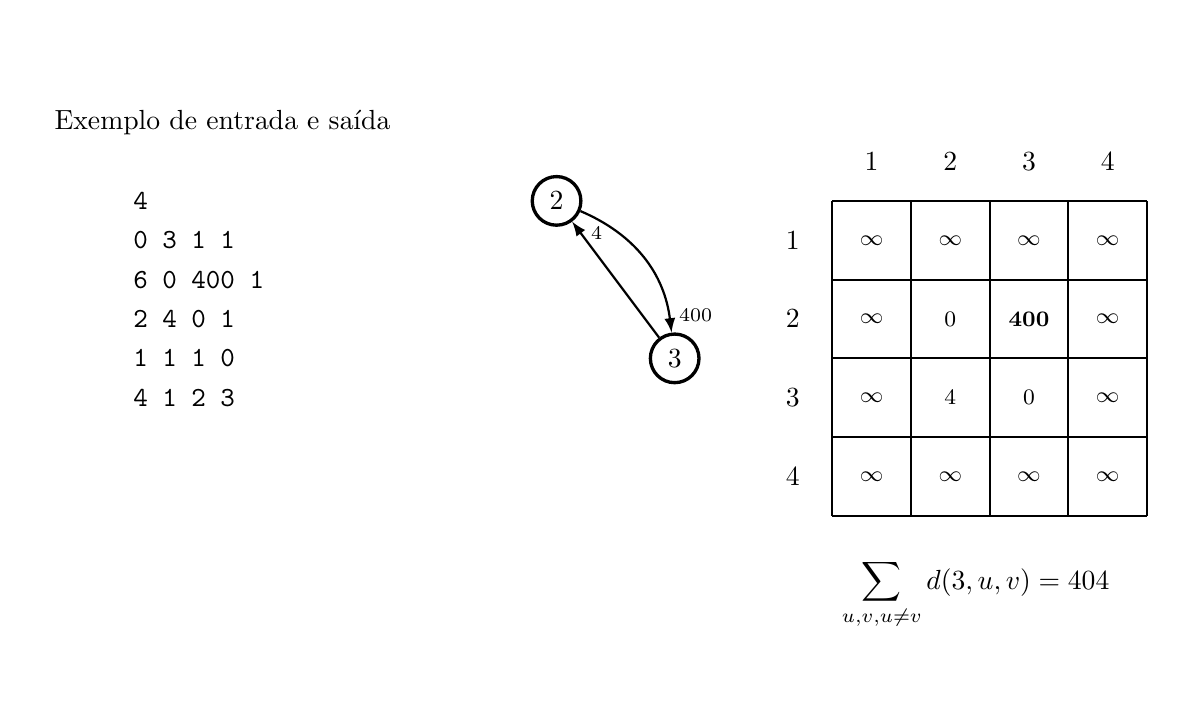
\begin{tikzpicture}
\node[draw,opacity=0] at (0, 0) {x};
\node[draw,opacity=0] at (14, 8) {x};

	\node[anchor=west] (header) at (0, 7.0) { \bbbold{Exemplo de entrada e saída} };


	\node[anchor=west] (line1) at (1.0, 6.0) { \bbtext{\texttt{4} } };



	\node[draw,very thick,circle] (node2) at (6.5, 6.0) { \bbtext{2} };

	\node[draw,very thick,circle] (node3) at (8.0, 4.0) { \bbtext{3} };



	\node[anchor=west] (line2) at (1.0, 5.5) { \bbtext{\texttt{0 3 1 1} } };

	\node[anchor=west] (line3) at (1.0, 5.0) { \bbtext{\texttt{6 0 400 1} } };

	\node[anchor=west] (line4) at (1.0, 4.5) { \bbtext{\texttt{2 4 0 1} } };

	\node[anchor=west] (line5) at (1.0, 4.0) { \bbtext{\texttt{1 1 1 0} } };


	\draw[thick] (10.0, 2.0) grid  (14.0, 6.0);

	\node[] (c1) at (9.5, 5.5) { \bbtext{1} };

	\node[] (c2) at (9.5, 4.5) { \bbtext{2} };

	\node[] (c3) at (9.5, 3.5) { \bbtext{3} };

	\node[] (c4) at (9.5, 2.5) { \bbtext{4} };

	\node[] (r1) at (10.5, 6.5) { \bbtext{1} };

	\node[] (r2) at (11.5, 6.5) { \bbtext{2} };

	\node[] (r3) at (12.5, 6.5) { \bbtext{3} };

	\node[] (r4) at (13.5, 6.5) { \bbtext{4} };

	\node[] (a11) at (10.5, 5.5) { \footnotesize $\infty$ };

	\node[] (a12) at (11.5, 5.5) { \footnotesize $\infty$ };

	\node[] (a13) at (12.5, 5.5) { \footnotesize $\infty$ };

	\node[] (a14) at (13.5, 5.5) { \footnotesize $\infty$ };

	\node[] (a21) at (10.5, 4.5) { \footnotesize $\infty$ };

	\node[] (a22) at (11.5, 4.5) { \footnotesize $0$ };

	\node[] (a23) at (12.5, 4.5) { \footnotesize $\mathbf{400}$ };

	\node[] (a24) at (13.5, 4.5) { \footnotesize $\infty$ };

	\node[] (a31) at (10.5, 3.5) { \footnotesize $\infty$ };

	\node[] (a32) at (11.5, 3.5) { \footnotesize ${4}$ };

	\node[] (a33) at (12.5, 3.5) { \footnotesize $0$ };

	\node[] (a34) at (13.5, 3.5) { \footnotesize $\infty$ };

	\node[] (a41) at (10.5, 2.5) { \footnotesize $\infty$ };

	\node[] (a42) at (11.5, 2.5) { \footnotesize $\infty$ };

	\node[] (a43) at (12.5, 2.5) { \footnotesize $\infty$ };

	\node[] (a44) at (13.5, 2.5) { \footnotesize $\infty$ };





	\draw[-latex,thick](node2) to [bend left] node[right,pos=0.9] { \scriptsize \bbinfo{400} } (node3);



	\draw[-latex,thick](node3) to node[right,pos=0.9] { \scriptsize \bbinfo{4} } (node2);







	\node[anchor=west] (line6) at (1.0, 3.5) { \bbtext{\texttt{4 1 2 3} } };




	\node[anchor=west] (eq) at (10.0, 1.0) { $\displaystyle \sum_{u, v, u\neq v} d(3, u, v) = 404$ };





















\end{tikzpicture}
\end{frame}
\begin{frame}[plain,t]
\begin{tikzpicture}
\node[draw,opacity=0] at (0, 0) {x};
\node[draw,opacity=0] at (14, 8) {x};

	\node[anchor=west] (header) at (0, 7.0) { \bbbold{Exemplo de entrada e saída} };


	\node[anchor=west] (line1) at (1.0, 6.0) { \bbtext{\texttt{4} } };



	\node[draw,very thick,circle,fill=BBRed] (node2) at (6.5, 6.0) { \bbtext{2} };

	\node[draw,very thick,circle] (node3) at (8.0, 4.0) { \bbtext{3} };



	\node[anchor=west] (line2) at (1.0, 5.5) { \bbtext{\texttt{0 3 1 1} } };

	\node[anchor=west] (line3) at (1.0, 5.0) { \bbtext{\texttt{6 0 400 1} } };

	\node[anchor=west] (line4) at (1.0, 4.5) { \bbtext{\texttt{2 4 0 1} } };

	\node[anchor=west] (line5) at (1.0, 4.0) { \bbtext{\texttt{1 1 1 0} } };


	\draw[thick] (10.0, 2.0) grid  (14.0, 6.0);

	\node[] (c1) at (9.5, 5.5) { \bbtext{1} };

	\node[] (c2) at (9.5, 4.5) { \bbtext{2} };

	\node[] (c3) at (9.5, 3.5) { \bbtext{3} };

	\node[] (c4) at (9.5, 2.5) { \bbtext{4} };

	\node[] (r1) at (10.5, 6.5) { \bbtext{1} };

	\node[] (r2) at (11.5, 6.5) { \bbtext{2} };

	\node[] (r3) at (12.5, 6.5) { \bbtext{3} };

	\node[] (r4) at (13.5, 6.5) { \bbtext{4} };

	\node[] (a11) at (10.5, 5.5) { \footnotesize $\infty$ };

	\node[] (a12) at (11.5, 5.5) { \footnotesize $\infty$ };

	\node[] (a13) at (12.5, 5.5) { \footnotesize $\infty$ };

	\node[] (a14) at (13.5, 5.5) { \footnotesize $\infty$ };

	\node[] (a21) at (10.5, 4.5) { \footnotesize $\infty$ };

	\node[] (a22) at (11.5, 4.5) { \footnotesize $0$ };

	\node[] (a23) at (12.5, 4.5) { \footnotesize ${400}$ };

	\node[] (a24) at (13.5, 4.5) { \footnotesize $\infty$ };

	\node[] (a31) at (10.5, 3.5) { \footnotesize $\infty$ };

	\node[] (a32) at (11.5, 3.5) { \footnotesize ${4}$ };

	\node[] (a33) at (12.5, 3.5) { \footnotesize $0$ };

	\node[] (a34) at (13.5, 3.5) { \footnotesize $\infty$ };

	\node[] (a41) at (10.5, 2.5) { \footnotesize $\infty$ };

	\node[] (a42) at (11.5, 2.5) { \footnotesize $\infty$ };

	\node[] (a43) at (12.5, 2.5) { \footnotesize $\infty$ };

	\node[] (a44) at (13.5, 2.5) { \footnotesize $\infty$ };





	\draw[-latex,thick](node2) to [bend left] node[right,pos=0.9] { \scriptsize \bbinfo{400} } (node3);



	\draw[-latex,thick](node3) to node[right,pos=0.9] { \scriptsize \bbinfo{4} } (node2);







	\node[anchor=west] (line6) at (1.0, 3.5) { \bbtext{\texttt{4 1 2 3} } };





























\end{tikzpicture}
\end{frame}
\begin{frame}[plain,t]
\begin{tikzpicture}
\node[draw,opacity=0] at (0, 0) {x};
\node[draw,opacity=0] at (14, 8) {x};

	\node[anchor=west] (header) at (0, 7.0) { \bbbold{Exemplo de entrada e saída} };


	\node[anchor=west] (line1) at (1.0, 6.0) { \bbtext{\texttt{4} } };




	\node[draw,very thick,circle] (node3) at (8.0, 4.0) { \bbtext{3} };



	\node[anchor=west] (line2) at (1.0, 5.5) { \bbtext{\texttt{0 3 1 1} } };

	\node[anchor=west] (line3) at (1.0, 5.0) { \bbtext{\texttt{6 0 400 1} } };

	\node[anchor=west] (line4) at (1.0, 4.5) { \bbtext{\texttt{2 4 0 1} } };

	\node[anchor=west] (line5) at (1.0, 4.0) { \bbtext{\texttt{1 1 1 0} } };


	\draw[thick] (10.0, 2.0) grid  (14.0, 6.0);

	\node[] (c1) at (9.5, 5.5) { \bbtext{1} };

	\node[] (c2) at (9.5, 4.5) { \bbtext{2} };

	\node[] (c3) at (9.5, 3.5) { \bbtext{3} };

	\node[] (c4) at (9.5, 2.5) { \bbtext{4} };

	\node[] (r1) at (10.5, 6.5) { \bbtext{1} };

	\node[] (r2) at (11.5, 6.5) { \bbtext{2} };

	\node[] (r3) at (12.5, 6.5) { \bbtext{3} };

	\node[] (r4) at (13.5, 6.5) { \bbtext{4} };

	\node[] (a11) at (10.5, 5.5) { \footnotesize $\infty$ };

	\node[] (a12) at (11.5, 5.5) { \footnotesize $\infty$ };

	\node[] (a13) at (12.5, 5.5) { \footnotesize $\infty$ };

	\node[] (a14) at (13.5, 5.5) { \footnotesize $\infty$ };

	\node[] (a21) at (10.5, 4.5) { \footnotesize $\infty$ };

	\node[] (a22) at (11.5, 4.5) { \footnotesize $0$ };

	\node[] (a23) at (12.5, 4.5) { \footnotesize ${400}$ };

	\node[] (a24) at (13.5, 4.5) { \footnotesize $\infty$ };

	\node[] (a31) at (10.5, 3.5) { \footnotesize $\infty$ };

	\node[] (a32) at (11.5, 3.5) { \footnotesize ${4}$ };

	\node[] (a33) at (12.5, 3.5) { \footnotesize $0$ };

	\node[] (a34) at (13.5, 3.5) { \footnotesize $\infty$ };

	\node[] (a41) at (10.5, 2.5) { \footnotesize $\infty$ };

	\node[] (a42) at (11.5, 2.5) { \footnotesize $\infty$ };

	\node[] (a43) at (12.5, 2.5) { \footnotesize $\infty$ };

	\node[] (a44) at (13.5, 2.5) { \footnotesize $\infty$ };















	\node[anchor=west] (line6) at (1.0, 3.5) { \bbtext{\texttt{4 1 2 3} } };































\end{tikzpicture}
\end{frame}
\begin{frame}[plain,t]
\begin{tikzpicture}
\node[draw,opacity=0] at (0, 0) {x};
\node[draw,opacity=0] at (14, 8) {x};

	\node[anchor=west] (header) at (0, 7.0) { \bbbold{Exemplo de entrada e saída} };


	\node[anchor=west] (line1) at (1.0, 6.0) { \bbtext{\texttt{4} } };




	\node[draw,very thick,circle] (node3) at (8.0, 4.0) { \bbtext{3} };



	\node[anchor=west] (line2) at (1.0, 5.5) { \bbtext{\texttt{0 3 1 1} } };

	\node[anchor=west] (line3) at (1.0, 5.0) { \bbtext{\texttt{6 0 400 1} } };

	\node[anchor=west] (line4) at (1.0, 4.5) { \bbtext{\texttt{2 4 0 1} } };

	\node[anchor=west] (line5) at (1.0, 4.0) { \bbtext{\texttt{1 1 1 0} } };


	\draw[thick] (10.0, 2.0) grid  (14.0, 6.0);

	\node[] (c1) at (9.5, 5.5) { \bbtext{1} };

	\node[] (c2) at (9.5, 4.5) { \bbtext{2} };

	\node[] (c3) at (9.5, 3.5) { \bbtext{3} };

	\node[] (c4) at (9.5, 2.5) { \bbtext{4} };

	\node[] (r1) at (10.5, 6.5) { \bbtext{1} };

	\node[] (r2) at (11.5, 6.5) { \bbtext{2} };

	\node[] (r3) at (12.5, 6.5) { \bbtext{3} };

	\node[] (r4) at (13.5, 6.5) { \bbtext{4} };

	\node[] (a11) at (10.5, 5.5) { \footnotesize $\infty$ };

	\node[] (a12) at (11.5, 5.5) { \footnotesize $\infty$ };

	\node[] (a13) at (12.5, 5.5) { \footnotesize $\infty$ };

	\node[] (a14) at (13.5, 5.5) { \footnotesize $\infty$ };

	\node[] (a21) at (10.5, 4.5) { \footnotesize $\infty$ };

	\node[] (a22) at (11.5, 4.5) { \footnotesize $\infty$ };

	\node[] (a23) at (12.5, 4.5) { \footnotesize $\infty$ };

	\node[] (a24) at (13.5, 4.5) { \footnotesize $\infty$ };

	\node[] (a31) at (10.5, 3.5) { \footnotesize $\infty$ };

	\node[] (a32) at (11.5, 3.5) { \footnotesize $\infty$ };

	\node[] (a33) at (12.5, 3.5) { \footnotesize $0$ };

	\node[] (a34) at (13.5, 3.5) { \footnotesize $\infty$ };

	\node[] (a41) at (10.5, 2.5) { \footnotesize $\infty$ };

	\node[] (a42) at (11.5, 2.5) { \footnotesize $\infty$ };

	\node[] (a43) at (12.5, 2.5) { \footnotesize $\infty$ };

	\node[] (a44) at (13.5, 2.5) { \footnotesize $\infty$ };















	\node[anchor=west] (line6) at (1.0, 3.5) { \bbtext{\texttt{4 1 2 3} } };

































\end{tikzpicture}
\end{frame}
\begin{frame}[plain,t]
\begin{tikzpicture}
\node[draw,opacity=0] at (0, 0) {x};
\node[draw,opacity=0] at (14, 8) {x};

	\node[anchor=west] (header) at (0, 7.0) { \bbbold{Exemplo de entrada e saída} };


	\node[anchor=west] (line1) at (1.0, 6.0) { \bbtext{\texttt{4} } };




	\node[draw,very thick,circle] (node3) at (8.0, 4.0) { \bbtext{3} };



	\node[anchor=west] (line2) at (1.0, 5.5) { \bbtext{\texttt{0 3 1 1} } };

	\node[anchor=west] (line3) at (1.0, 5.0) { \bbtext{\texttt{6 0 400 1} } };

	\node[anchor=west] (line4) at (1.0, 4.5) { \bbtext{\texttt{2 4 0 1} } };

	\node[anchor=west] (line5) at (1.0, 4.0) { \bbtext{\texttt{1 1 1 0} } };


	\draw[thick] (10.0, 2.0) grid  (14.0, 6.0);

	\node[] (c1) at (9.5, 5.5) { \bbtext{1} };

	\node[] (c2) at (9.5, 4.5) { \bbtext{2} };

	\node[] (c3) at (9.5, 3.5) { \bbtext{3} };

	\node[] (c4) at (9.5, 2.5) { \bbtext{4} };

	\node[] (r1) at (10.5, 6.5) { \bbtext{1} };

	\node[] (r2) at (11.5, 6.5) { \bbtext{2} };

	\node[] (r3) at (12.5, 6.5) { \bbtext{3} };

	\node[] (r4) at (13.5, 6.5) { \bbtext{4} };

	\node[] (a11) at (10.5, 5.5) { \footnotesize $\infty$ };

	\node[] (a12) at (11.5, 5.5) { \footnotesize $\infty$ };

	\node[] (a13) at (12.5, 5.5) { \footnotesize $\infty$ };

	\node[] (a14) at (13.5, 5.5) { \footnotesize $\infty$ };

	\node[] (a21) at (10.5, 4.5) { \footnotesize $\infty$ };

	\node[] (a22) at (11.5, 4.5) { \footnotesize $\infty$ };

	\node[] (a23) at (12.5, 4.5) { \footnotesize $\infty$ };

	\node[] (a24) at (13.5, 4.5) { \footnotesize $\infty$ };

	\node[] (a31) at (10.5, 3.5) { \footnotesize $\infty$ };

	\node[] (a32) at (11.5, 3.5) { \footnotesize $\infty$ };

	\node[] (a33) at (12.5, 3.5) { \footnotesize $0$ };

	\node[] (a34) at (13.5, 3.5) { \footnotesize $\infty$ };

	\node[] (a41) at (10.5, 2.5) { \footnotesize $\infty$ };

	\node[] (a42) at (11.5, 2.5) { \footnotesize $\infty$ };

	\node[] (a43) at (12.5, 2.5) { \footnotesize $\infty$ };

	\node[] (a44) at (13.5, 2.5) { \footnotesize $\infty$ };















	\node[anchor=west] (line6) at (1.0, 3.5) { \bbtext{\texttt{4 1 2 3} } };




	\node[anchor=west] (eq) at (10.0, 1.0) { $\displaystyle \sum_{u, v, u\neq v} d(4, u, v) = 0$ };
































\end{tikzpicture}
\end{frame}
\begin{frame}[plain,t]
\begin{tikzpicture}
\node[draw,opacity=0] at (0, 0) {x};
\node[draw,opacity=0] at (14, 8) {x};

	\node[anchor=west] (header) at (0, 7.0) { \bbbold{Exemplo de entrada e saída} };


	\node[anchor=west] (line1) at (1.0, 6.0) { \bbtext{\texttt{4} } };




	\node[draw,very thick,circle] (node3) at (8.0, 4.0) { \bbtext{3} };



	\node[anchor=west] (line2) at (1.0, 5.5) { \bbtext{\texttt{0 3 1 1} } };

	\node[anchor=west] (line3) at (1.0, 5.0) { \bbtext{\texttt{6 0 400 1} } };

	\node[anchor=west] (line4) at (1.0, 4.5) { \bbtext{\texttt{2 4 0 1} } };

	\node[anchor=west] (line5) at (1.0, 4.0) { \bbtext{\texttt{1 1 1 0} } };


	\draw[thick] (10.0, 2.0) grid  (14.0, 6.0);

	\node[] (c1) at (9.5, 5.5) { \bbtext{1} };

	\node[] (c2) at (9.5, 4.5) { \bbtext{2} };

	\node[] (c3) at (9.5, 3.5) { \bbtext{3} };

	\node[] (c4) at (9.5, 2.5) { \bbtext{4} };

	\node[] (r1) at (10.5, 6.5) { \bbtext{1} };

	\node[] (r2) at (11.5, 6.5) { \bbtext{2} };

	\node[] (r3) at (12.5, 6.5) { \bbtext{3} };

	\node[] (r4) at (13.5, 6.5) { \bbtext{4} };

	\node[] (a11) at (10.5, 5.5) { \footnotesize $\infty$ };

	\node[] (a12) at (11.5, 5.5) { \footnotesize $\infty$ };

	\node[] (a13) at (12.5, 5.5) { \footnotesize $\infty$ };

	\node[] (a14) at (13.5, 5.5) { \footnotesize $\infty$ };

	\node[] (a21) at (10.5, 4.5) { \footnotesize $\infty$ };

	\node[] (a22) at (11.5, 4.5) { \footnotesize $\infty$ };

	\node[] (a23) at (12.5, 4.5) { \footnotesize $\infty$ };

	\node[] (a24) at (13.5, 4.5) { \footnotesize $\infty$ };

	\node[] (a31) at (10.5, 3.5) { \footnotesize $\infty$ };

	\node[] (a32) at (11.5, 3.5) { \footnotesize $\infty$ };

	\node[] (a33) at (12.5, 3.5) { \footnotesize $0$ };

	\node[] (a34) at (13.5, 3.5) { \footnotesize $\infty$ };

	\node[] (a41) at (10.5, 2.5) { \footnotesize $\infty$ };

	\node[] (a42) at (11.5, 2.5) { \footnotesize $\infty$ };

	\node[] (a43) at (12.5, 2.5) { \footnotesize $\infty$ };

	\node[] (a44) at (13.5, 2.5) { \footnotesize $\infty$ };















	\node[anchor=west] (line6) at (1.0, 3.5) { \bbtext{\texttt{4 1 2 3} } };




	\node[anchor=west] (eq) at (10.0, 1.0) { $\displaystyle \sum_{u, v, u\neq v} d(4, u, v) = 0$ };

































	\draw[-latex,very thick,color=BBBlack] (1.85, 3.25) to  (1.85, 2.25);

	\node[] (r) at (1.85, 2.0) { \footnotesize \bboutput{17 23 404 0} };

\end{tikzpicture}
\end{frame}
\begin{frame}[plain,t]
\begin{tikzpicture}
\node[draw,opacity=0] at (0, 0) {x};
\node[draw,opacity=0] at (14, 8) {x};

	\node[anchor=west] (header) at (0.0, 7.0) { \Large \bbbold{Solução} };

\end{tikzpicture}
\end{frame}
\begin{frame}[plain,t]
\begin{tikzpicture}
\node[draw,opacity=0] at (0, 0) {x};
\node[draw,opacity=0] at (14, 8) {x};

	\node[anchor=west] (header) at (0.0, 7.0) { \Large \bbbold{Solução} };


	\node[anchor=west] (line1) at (1.0, 6.0) { $\star$ \bbtext{As arestas de um vértice podem ser removidas da matriz de adjacências} };

	\node[anchor=west] (line1a) at (0.5, 5.5) { \bbtext{em $O(N)$} };

\end{tikzpicture}
\end{frame}
\begin{frame}[plain,t]
\begin{tikzpicture}
\node[draw,opacity=0] at (0, 0) {x};
\node[draw,opacity=0] at (14, 8) {x};

	\node[anchor=west] (header) at (0.0, 7.0) { \Large \bbbold{Solução} };


	\node[anchor=west] (line1) at (1.0, 6.0) { $\star$ \bbtext{As arestas de um vértice podem ser removidas da matriz de adjacências} };

	\node[anchor=west] (line1a) at (0.5, 5.5) { \bbtext{em $O(N)$} };


	\node[anchor=west] (line2) at (1.0, 4.5) { $\star$ \bbtext{Em cada etapa, os caminhos mínimos entre todos os pares podem ser} };

	\node[anchor=west] (line2a) at (0.5, 4.0) { \bbtext{computados com Floyd-Warshall em $O(N^3)$} };

\end{tikzpicture}
\end{frame}
\begin{frame}[plain,t]
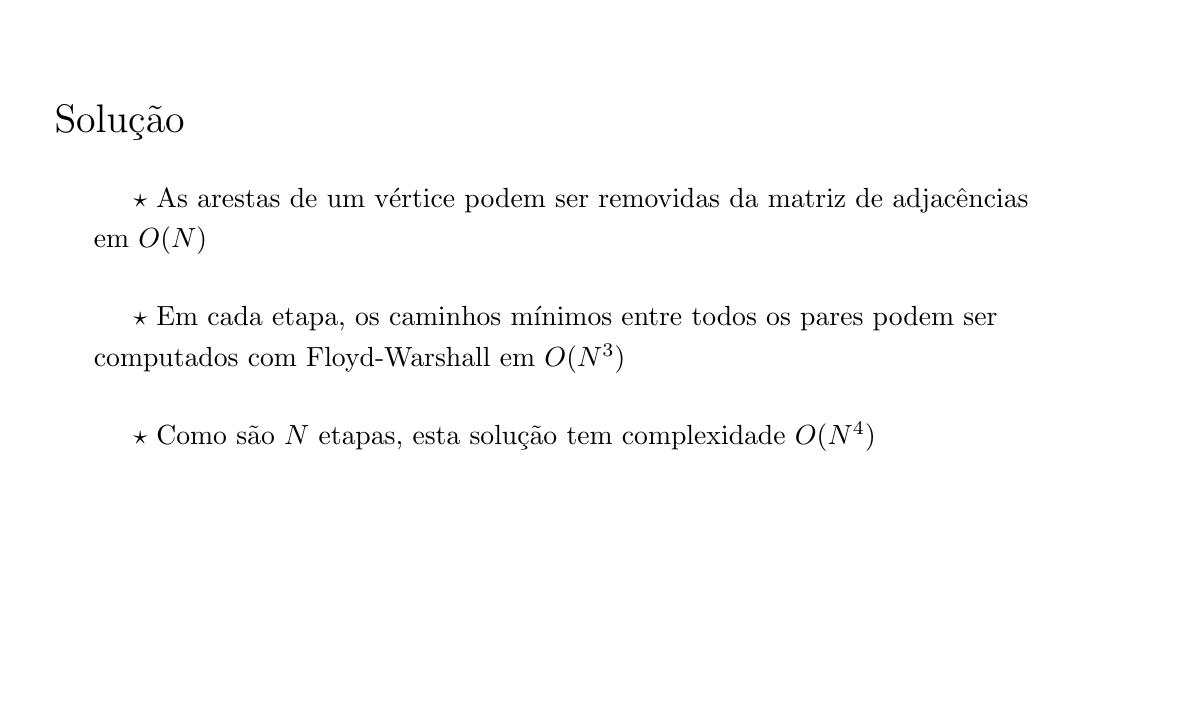
\begin{tikzpicture}
\node[draw,opacity=0] at (0, 0) {x};
\node[draw,opacity=0] at (14, 8) {x};

	\node[anchor=west] (header) at (0.0, 7.0) { \Large \bbbold{Solução} };


	\node[anchor=west] (line1) at (1.0, 6.0) { $\star$ \bbtext{As arestas de um vértice podem ser removidas da matriz de adjacências} };

	\node[anchor=west] (line1a) at (0.5, 5.5) { \bbtext{em $O(N)$} };


	\node[anchor=west] (line2) at (1.0, 4.5) { $\star$ \bbtext{Em cada etapa, os caminhos mínimos entre todos os pares podem ser} };

	\node[anchor=west] (line2a) at (0.5, 4.0) { \bbtext{computados com Floyd-Warshall em $O(N^3)$} };


	\node[anchor=west] (line3) at (1.0, 3.0) { $\star$ \bbtext{Como são $N$ etapas, esta solução tem complexidade $O(N^4)$} };
\end{tikzpicture}
\end{frame}
\begin{frame}[plain,t]
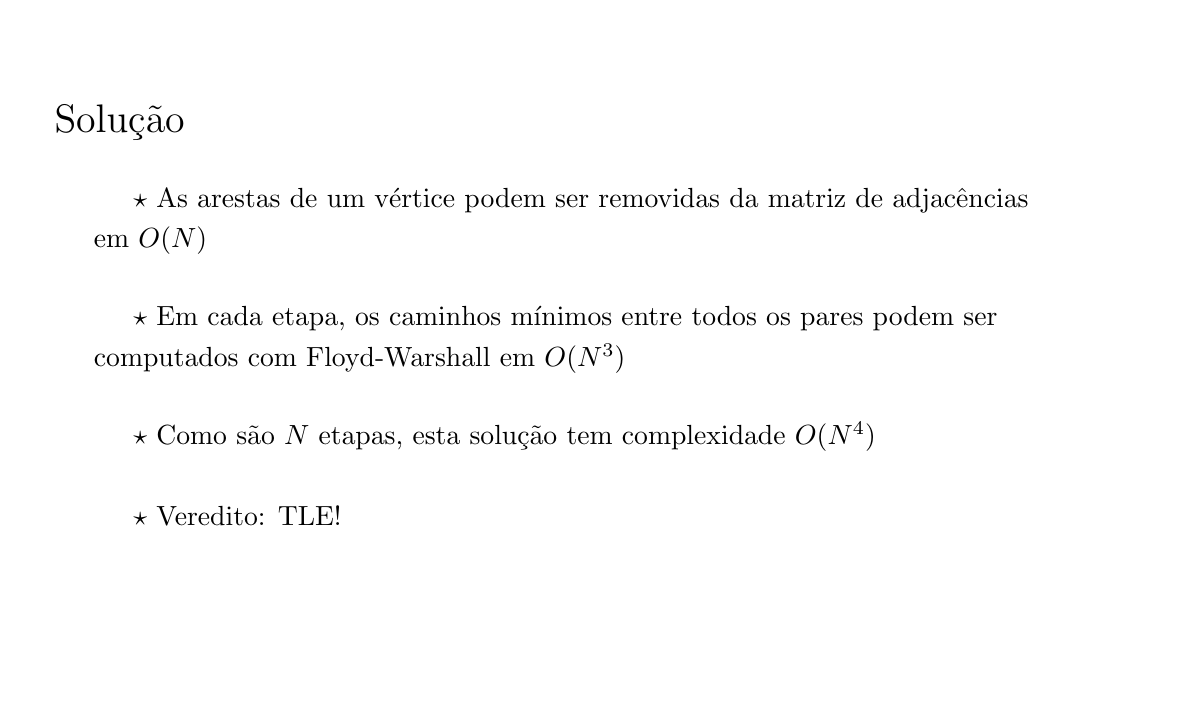
\begin{tikzpicture}
\node[draw,opacity=0] at (0, 0) {x};
\node[draw,opacity=0] at (14, 8) {x};

	\node[anchor=west] (header) at (0.0, 7.0) { \Large \bbbold{Solução} };


	\node[anchor=west] (line1) at (1.0, 6.0) { $\star$ \bbtext{As arestas de um vértice podem ser removidas da matriz de adjacências} };

	\node[anchor=west] (line1a) at (0.5, 5.5) { \bbtext{em $O(N)$} };


	\node[anchor=west] (line2) at (1.0, 4.5) { $\star$ \bbtext{Em cada etapa, os caminhos mínimos entre todos os pares podem ser} };

	\node[anchor=west] (line2a) at (0.5, 4.0) { \bbtext{computados com Floyd-Warshall em $O(N^3)$} };


	\node[anchor=west] (line3) at (1.0, 3.0) { $\star$ \bbtext{Como são $N$ etapas, esta solução tem complexidade $O(N^4)$} };

	\node[anchor=west] (line4) at (1.0, 2.0) { $\star$ \bbbold{Veredito}\bbtext{: TLE!} };

\end{tikzpicture}
\end{frame}
\begin{frame}[plain,t]
\begin{tikzpicture}
\node[draw,opacity=0] at (0, 0) {x};
\node[draw,opacity=0] at (14, 8) {x};

	\node[anchor=west] (header) at (0.0, 7.0) { \Large \bbbold{Solução} };


	\node[anchor=west] (line1) at (1.0, 6.0) { $\star$ \bbtext{Para reduzir a complexidade, é preciso compreender o funcionamento do} };

	\node[anchor=west] (line1a) at (0.5, 5.5) { \bbtext{algoritmo de Floyd-Warshall} };

\end{tikzpicture}
\end{frame}
\begin{frame}[plain,t]
\begin{tikzpicture}
\node[draw,opacity=0] at (0, 0) {x};
\node[draw,opacity=0] at (14, 8) {x};

	\node[anchor=west] (header) at (0.0, 7.0) { \Large \bbbold{Solução} };


	\node[anchor=west] (line1) at (1.0, 6.0) { $\star$ \bbtext{Para reduzir a complexidade, é preciso compreender o funcionamento do} };

	\node[anchor=west] (line1a) at (0.5, 5.5) { \bbtext{algoritmo de Floyd-Warshall} };


	\node[anchor=west] (line2) at (1.0, 4.5) { $\star$ \bbtext{A cada iteração, as distâncias são relaxadas usando o vértice $k$ como} };

	\node[anchor=west] (line2a) at (0.5, 4.0) { \bbtext{intermediário} };

\end{tikzpicture}
\end{frame}
\begin{frame}[plain,t]
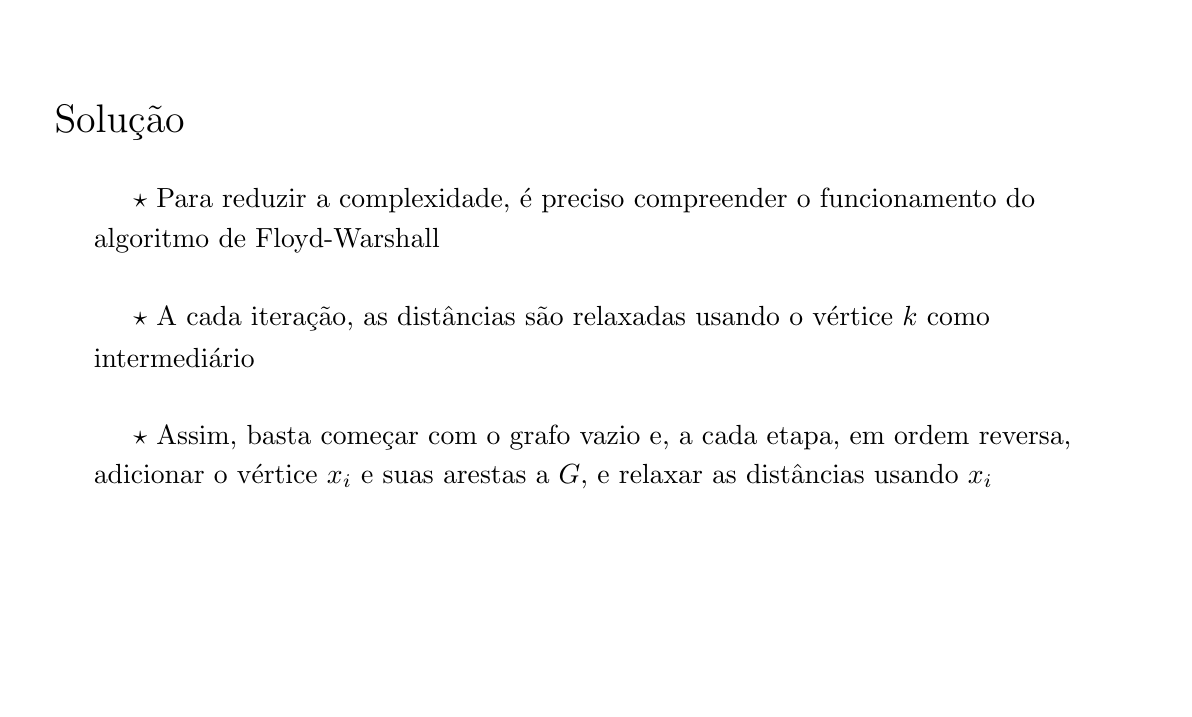
\begin{tikzpicture}
\node[draw,opacity=0] at (0, 0) {x};
\node[draw,opacity=0] at (14, 8) {x};

	\node[anchor=west] (header) at (0.0, 7.0) { \Large \bbbold{Solução} };


	\node[anchor=west] (line1) at (1.0, 6.0) { $\star$ \bbtext{Para reduzir a complexidade, é preciso compreender o funcionamento do} };

	\node[anchor=west] (line1a) at (0.5, 5.5) { \bbtext{algoritmo de Floyd-Warshall} };


	\node[anchor=west] (line2) at (1.0, 4.5) { $\star$ \bbtext{A cada iteração, as distâncias são relaxadas usando o vértice $k$ como} };

	\node[anchor=west] (line2a) at (0.5, 4.0) { \bbtext{intermediário} };


	\node[anchor=west] (line3) at (1.0, 3.0) { $\star$ \bbtext{Assim, basta começar com o grafo vazio e, a cada etapa, em ordem reversa,} };

	\node[anchor=west] (line3a) at (0.5, 2.5) { \bbtext{adicionar o vértice $x_i$ e suas arestas a $G$, e relaxar as distâncias usando $x_i$} };

\end{tikzpicture}
\end{frame}
\begin{frame}[plain,t]
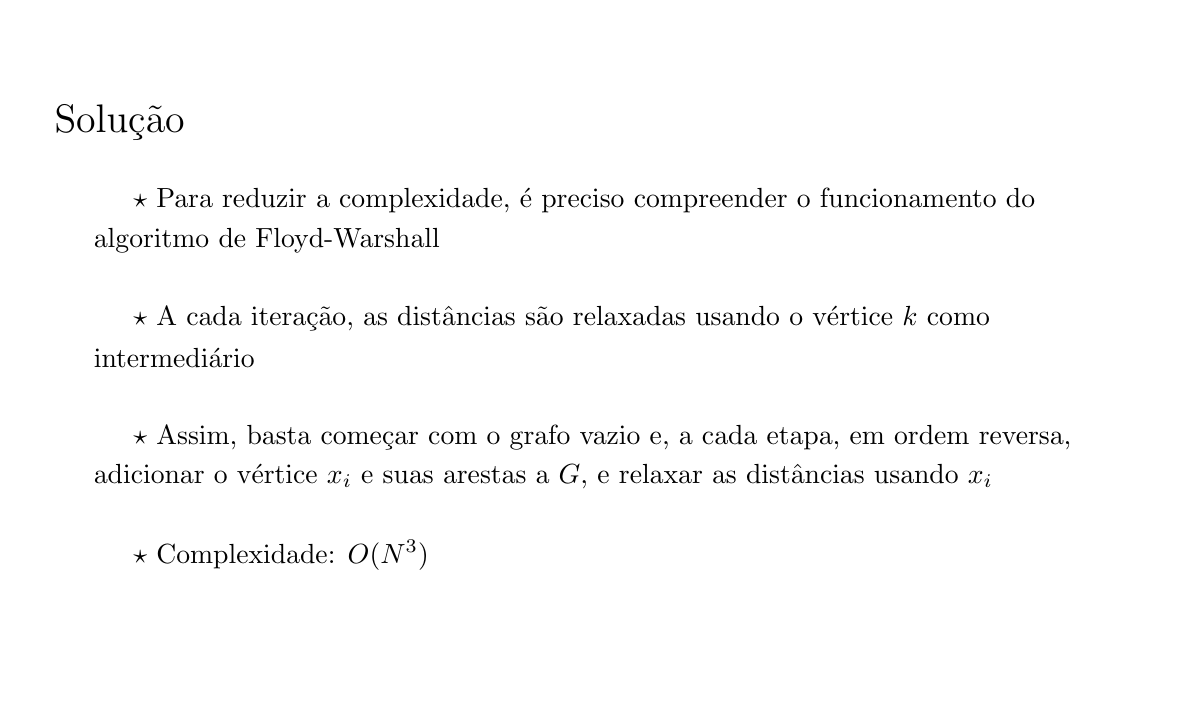
\begin{tikzpicture}
\node[draw,opacity=0] at (0, 0) {x};
\node[draw,opacity=0] at (14, 8) {x};

	\node[anchor=west] (header) at (0.0, 7.0) { \Large \bbbold{Solução} };


	\node[anchor=west] (line1) at (1.0, 6.0) { $\star$ \bbtext{Para reduzir a complexidade, é preciso compreender o funcionamento do} };

	\node[anchor=west] (line1a) at (0.5, 5.5) { \bbtext{algoritmo de Floyd-Warshall} };


	\node[anchor=west] (line2) at (1.0, 4.5) { $\star$ \bbtext{A cada iteração, as distâncias são relaxadas usando o vértice $k$ como} };

	\node[anchor=west] (line2a) at (0.5, 4.0) { \bbtext{intermediário} };


	\node[anchor=west] (line3) at (1.0, 3.0) { $\star$ \bbtext{Assim, basta começar com o grafo vazio e, a cada etapa, em ordem reversa,} };

	\node[anchor=west] (line3a) at (0.5, 2.5) { \bbtext{adicionar o vértice $x_i$ e suas arestas a $G$, e relaxar as distâncias usando $x_i$} };


	\node[anchor=west] (line4) at (1.0, 1.5) { $\star$ \bbbold{Complexidade}\bbtext{: $O(N^3)$} };


\end{tikzpicture}
\end{frame}
\begin{frame}[plain,t]

\inputsnippet{cpp}{11}{28}{codes/295B.cpp}

\end{frame}
\begin{frame}[plain,t]

\inputsnippet{cpp}{30}{42}{codes/295B.cpp}

\end{frame}
\end{document}
